% ===================================================================
% 正文部分 — 基于脑电运动想象的脑机接口系统研究
% ===================================================================

% ===================================================================
\section{绪论}
\label{sec:introduction}
% ===================================================================

% -------------------------------------------------------------------
\subsection{研究背景与意义}
\label{sec:background}
% -------------------------------------------------------------------

脑机接口（Brain-Computer Interface, BCI）是一种不依赖外周神经和肌肉组织、直接在大脑与外部设备之间建立通信通道的技术\upcite{wolpaw2002bci}。它通过采集、解析大脑活动信号，将使用者的意图转化为控制指令，从而驱动轮椅、拼写器或假肢等辅助设备。对于因肌萎缩侧索硬化（ALS）、脊髓损伤或中风等疾病导致严重运动障碍的患者而言，BCI 提供了一条绕过受损运动通路的替代通信途径\upcite{wolpaw2012bci}。据世界卫生组织统计，全球约有 13 亿人——占世界人口的 16\%——经历某种形式的残疾\upcite{who2023disability}，其中运动功能障碍占据相当比例。BCI 技术的发展不仅具有重要的科学研究价值，更对改善这一群体的生活质量具有深远的社会意义。

BCI 系统的一般工作流程可概括为四个环节：（1）\textbf{信号采集}——通过脑电（EEG）、脑磁图（MEG）或功能性近红外光谱（fNIRS）等手段记录大脑活动；（2）\textbf{信号处理}——对原始信号进行滤波、去噪、特征提取；（3）\textbf{模式识别}——利用机器学习算法将提取的特征映射为控制指令；（4）\textbf{反馈输出}——将识别结果转化为外部设备动作并向使用者提供实时反馈。在各类脑信号采集方式中，EEG 因其非侵入性、时间分辨率高（毫秒级）、设备成本低、便携性好，成为 BCI 研究中应用最广泛的信号模态\upcite{nicolas2012bci}。

在众多 BCI 范式中，运动想象（Motor Imagery, MI）是一种主动式范式——使用者无需借助外部视觉或听觉刺激，仅通过在头脑中想象肢体运动即可产生可区分的脑电特征\upcite{pfurtscheller1997mu}。这一特性使 MI-BCI 具有独立性强、操作自然的优势，被认为是最具临床应用潜力的 BCI 范式之一\upcite{wolpaw2012bci}。

% -------------------------------------------------------------------
\subsection{国内外研究现状}
\label{sec:related-work}
% -------------------------------------------------------------------

\subsubsection{基于空间滤波的传统方法}

共空间模式（Common Spatial Patterns, CSP）自 2000 年被引入运动想象 BCI 领域以来\upcite{ramoser2000csp}，迅速成为最主流的空间滤波与特征提取方法。CSP 通过广义特征值分解寻找一组空间滤波器，使滤波后信号在两类条件下的方差比值最大化，从而实现类别区分。Blankertz 等人在此基础上提出了多种改进方案，包括正则化 CSP 和鲁棒 CSP\upcite{blankertz2008csp}，以提高算法在噪声环境下的稳定性。

然而，标准 CSP 的性能高度依赖预滤波频段的选择。由于不同被试的最优判别频带存在显著个体差异——部分被试主要依赖 Mu 节律（8--13\,Hz），另一些则更多依赖 Beta 节律（13--30\,Hz）\upcite{blankertz2008csp}——固定频带的 CSP 难以实现最优性能。针对这一问题，Ang 等人提出了滤波器组共空间模式（Filter Bank CSP, FBCSP）\upcite{ang2008fbcsp}，将信号分解到多个子频带后独立提取 CSP 特征，再通过特征选择自动确定最佳频带组合。FBCSP 在 BCI Competition IV 中取得了冠军成绩\upcite{ang2012fbcsp}，验证了频带自适应机制的有效性。

\subsubsection{基于深度学习的方法}

近年来，深度学习方法也被引入 MI-BCI 领域\upcite{craik2019deep}。与传统方法需要手工设计特征工程流程不同，深度学习模型直接以原始 EEG 信号为输入，通过端到端学习自动提取判别特征。Schirrmeister 等人提出了 Deep ConvNet 和 Shallow ConvNet\upcite{schirrmeister2017deep}；Lawhern 等人设计了参数量极少（约 1,200 个）的轻量级模型 EEGNet\upcite{lawhern2018eegnet}，使其更适合 BCI 场景下的小样本学习。

然而，目前深度学习在 MI-BCI 中的表现并不一致\upcite{lotte2018review}。在数据量充足的场景下（如大规模跨被试训练），深度学习可能展现优势；但在单被试、小样本（通常仅 100--288 个试次）的典型 BCI 实验条件下，过参数化的深度模型容易过拟合，反而不如精心设计的传统空间滤波方法。这种"小数据困境"是深度学习在 MI-BCI 实际应用中面临的核心挑战。

\subsubsection{国内研究进展}

国内在脑机接口领域的研究起步较早且发展迅速。清华大学高小榕团队在基于稳态视觉诱发电位（SSVEP）的 BCI 系统方面取得了国际领先的成果，提出了高速 SSVEP 拼写器，信息传输率达到 5.32 bits/s\upcite{gao2014bci}。在运动想象方向，华东理工大学张宇团队将稀疏贝叶斯学习引入 CSP 频带特征选择，提出了基于稀疏优化的频带选择策略\upcite{zhang2019csp}，为 FBCSP 类方法提供了新的特征选择思路。此外，天津大学、上海交通大学、国防科技大学等机构也在运动想象解码、跨被试迁移学习和在线自适应方面开展了大量研究。近年来，国内 BCI 研究正从实验室阶段向临床应用转化，多所医院已开展基于 MI-BCI 的中风康复临床试验。

\subsubsection{现有方法面临的主要问题}

综合以上分析，当前 MI-BCI 研究主要面临以下问题：

\begin{enumerate}[leftmargin=2em]
	\item \textbf{频带选择的主观性。}标准 CSP 需要人为指定滤波频段，不同被试的最优频带差异大，缺乏自动化的频带选择机制。
	\item \textbf{跨被试泛化能力弱。}无论传统方法还是深度学习，单被试训练的模型难以直接迁移到其他被试，"BCI 盲"（BCI illiteracy）现象普遍存在\upcite{allison2010bciilliteracy}。
	\item \textbf{离线性能到在线部署的鸿沟。}大量研究停留在离线分析阶段，缺少从算法到完整在线系统的端到端实现验证。
\end{enumerate}

% -------------------------------------------------------------------
\subsection{本文研究内容}
\label{sec:research-content}
% -------------------------------------------------------------------

针对上述问题，本文围绕"基于脑电运动想象的脑机接口系统"展开研究，主要工作包括：

\begin{enumerate}[leftmargin=2em]
	\item \textbf{构建多方法对比框架。}实现 CSP+LDA（基线方法）、FBCSP+SVM（改进方法）和 EEGNet（深度学习探针）三条分类流水线，在统一的评估框架下进行公平对比。
	\item \textbf{验证 FBCSP 的频带自适应优势。}以 BCI Competition IV Dataset 2a 为主实验数据集，通过 10 折分层交叉验证和统计检验，定量分析 FBCSP+SVM 相对于 CSP+LDA 和 EEGNet 的性能差异。同时在 Dataset 2b 和 PhysioNet EEGBCI 数据集上进行泛化验证。
	\item \textbf{实现完整的在线仿真系统。}基于 WebSocket 协议搭建"数据回放 + 实时分类 + 浏览器反馈"的三层仿真架构，验证算法从离线评估到在线部署的可行性。
\end{enumerate}

% -------------------------------------------------------------------
\subsection{论文结构安排}
\label{sec:thesis-structure}
% -------------------------------------------------------------------

本文共分八章，各章内容安排如下：

\textbf{第一章 绪论}，介绍脑机接口的研究背景与意义，综述运动想象 BCI 的国内外研究现状，指出现有方法面临的关键问题，明确本文的研究内容。

\textbf{第二章 相关理论与技术基础}，阐述 EEG 信号的产生机制、运动想象的神经生理学基础（ERD/ERS），以及 CSP、FBCSP、LDA、SVM 和 EEGNet 的基本原理。

\textbf{第三章 系统总体设计}，介绍系统的两阶段架构（离线训练 + 在线仿真）、数据集参数、开发环境与技术选型，以及 YAML 配置驱动的实验管理方案。

\textbf{第四章 EEG 信号预处理}，详细描述从原始信号到分类就绪 epoch 的完整预处理流水线，包括共平均参考、带通滤波、ICA 伪迹去除、事件分段和坏段拒绝。

\textbf{第五章 特征提取与分类算法}，介绍三条分类流水线的具体实现：CSP+LDA 基线、FBCSP+SVM 改进方案和 EEGNet 深度学习探针。

\textbf{第六章 实验结果与分析}，在三个数据集上对比三种方法的分类性能，通过统计检验验证差异显著性，并从神经生理学角度分析被试间性能差异的原因。

\textbf{第七章 在线仿真系统实现}，基于第六章的算法选型结论，实现 WebSocket 三层架构的在线 BCI 仿真系统，验证从离线模型到在线部署的无损迁移。

\textbf{第八章 总结与展望}，总结本文的主要工作与贡献，分析不足之处，并展望未来的研究方向。


% ===================================================================
\section{相关理论与技术基础}
\label{sec:theory}
% ===================================================================

本章介绍运动想象脑机接口系统所涉及的基础理论。首先阐述脑电信号的产生机制与基本特性，然后从神经生理学角度解释运动想象的脑电特征，最后分别介绍共空间模式（CSP）、滤波器组共空间模式（FBCSP）、线性判别分析（LDA）、支持向量机（SVM）和 EEGNet 卷积神经网络的基本原理。这些理论构成第五章算法实现和第六章实验分析的基础。

% -------------------------------------------------------------------
\subsection{脑电信号基础}
\label{sec:eeg-basics}
% -------------------------------------------------------------------

\subsubsection{脑电信号的产生机制}

脑电图（Electroencephalography, EEG）记录的是大脑皮层大量锥体神经元突触后电位的同步叠加\upcite{niedermeyer2004eeg}。单个神经元的电活动极为微弱，只有当数以万计的神经元在时间上近似同步放电时，其产生的等效电偶极子才能在头皮表面被检测到。因此，EEG 信号本质上反映的是\textbf{大规模神经元群体的同步活动程度}，而非单个神经元的放电。

头皮采集的 EEG 信号幅值通常在 10--100\,$\mu$V 范围内，远小于心电信号（$\sim$1\,mV）和肌电信号（$\sim$10\,mV），信噪比极低。信号在穿过脑脊液、颅骨和头皮等组织时会经历严重的容积传导效应\upcite{nunez2006eeg}，导致空间分辨率有限（厘米级）——这意味着每个电极实际记录的是其下方较大区域皮层活动的空间平均，而非精确的点源信号。

\subsubsection{电极放置标准}

EEG 电极的放置遵循国际 10-20 系统标准\upcite{jasper195810-20}。该系统以颅骨解剖标志点（鼻根、枕骨粗隆、左右耳前点）之间的距离为基准，按 10\% 和 20\% 的等分间隔确定电极位置，确保不同实验室之间的可比性。

电极命名规则中，字母表示所覆盖的脑区：F（额叶）、C（中央区）、P（顶叶）、O（枕叶）、T（颞叶）；奇数编号对应左半球，偶数对应右半球，z 表示中线。对于运动想象 BCI 而言，最关键的电极是 \textbf{C3}（左侧运动皮层上方）和 \textbf{C4}（右侧运动皮层上方），因为运动想象的神经活动主要发生在对侧初级运动皮层区域。

\subsubsection{脑电节律}

EEG 信号可按频率分解为多种节律成分，每种节律与不同的脑功能状态相关\upcite{niedermeyer2004eeg}。表\ref{tab:rhythms}列出了主要的脑电节律。

\begin{table}[htbp]
	\centering
	\bicaption{主要脑电节律的频段范围与功能意义\label{tab:rhythms}}{Major EEG rhythms: frequency bands and functional significance}
	\begin{tabular}{cccc}
		\toprule
		节律名称 & 频段 (Hz) & 主要分布区域 & 功能意义 \\
		\midrule
		Delta ($\delta$) & 0.5--4 & 广泛分布 & 深度睡眠 \\
		Theta ($\theta$) & 4--8 & 额叶、颞叶 & 困倦、记忆编码 \\
		Alpha ($\alpha$) & 8--13 & 枕叶 & 清醒放松、闭眼静息 \\
		\textbf{Mu ($\mu$)} & \textbf{8--13} & \textbf{中央区 (C3/C4)} & \textbf{运动/运动想象相关} \\
		\textbf{Beta ($\beta$)} & \textbf{13--30} & \textbf{中央区、额叶} & \textbf{主动思维、运动控制} \\
		Gamma ($\gamma$) & $>$30 & 广泛分布 & 高级认知、特征绑定 \\
		\bottomrule
	\end{tabular}
\end{table}

其中，Mu 节律和 Beta 节律与运动想象脑机接口直接相关。Mu 节律与 Alpha 节律虽然频段重叠（均为 8--13\,Hz），但二者在头皮上的空间分布和功能意义不同：Alpha 节律主要分布在枕叶，与视觉注意相关；Mu 节律则特异性地分布在中央感觉运动区（C3/C4 附近），与运动控制和运动想象密切相关\upcite{pfurtscheller1999erds}。

% -------------------------------------------------------------------
\subsection{运动想象的神经生理学基础}
\label{sec:motor-imagery}
% -------------------------------------------------------------------

\subsubsection{运动想象的定义与神经基础}

运动想象（Motor Imagery, MI）是指在不产生实际肌肉运动的情况下，在心理上模拟特定运动动作的过程\upcite{jeannerod1995mental}。神经影像学研究表明，运动想象与实际运动执行共享大部分神经回路——初级运动皮层（M1）、辅助运动区（SMA）和前运动皮层（PMC）在运动想象时均被激活\upcite{pfurtscheller1997mu}。

这一发现为运动想象脑机接口提供了神经生理学基础：由于运动想象能够可靠地引起特定脑区的电活动变化，这些变化可以被 EEG 捕获并解码，从而实现不依赖肌肉活动的大脑-计算机通信。

\subsubsection{事件相关去同步与同步（ERD/ERS）}

运动想象引起的 EEG 变化主要表现为事件相关去同步（Event-Related Desynchronization, ERD）和事件相关同步（Event-Related Synchronization, ERS）\upcite{pfurtscheller1999erds}。

\textbf{ERD} 表现为特定频段脑电功率的\textbf{下降}，反映相关皮层区域神经元群体从同步状态转入去同步的活跃工作状态。\textbf{ERS} 则相反，表现为功率的\textbf{上升}，通常出现在运动结束后或不相关的脑区。

运动想象的 ERD/ERS 具有两个关键特性：

\textbf{（1）对侧优势。}想象移动左手时，右侧运动皮层（C4 电极附近）出现显著的 Mu/Beta ERD；想象移动右手时，则是左侧运动皮层（C3 电极附近）出现 ERD\upcite{mcfarland2000mu}。通俗地说，大脑控制运动的方式是"交叉"的——左脑管右手，右脑管左手——运动想象同样遵循这一规律。

\textbf{（2）频段特异性。}ERD 主要发生在 Mu（8--13\,Hz）和 Beta（13--30\,Hz）频段。不同被试对这两个频段的依赖程度不同：部分被试主要产生 Mu-ERD，另一些则更多依赖 Beta-ERD\upcite{blankertz2008csp}。这种个体差异是后续 FBCSP 方法的核心动机。

正是由于左/右手运动想象在空间（C3 vs C4）和频率（Mu/Beta ERD）上产生可区分的模式，EEG 信号才能被用于二分类 BCI 系统。本文的三种分类方法——CSP、FBCSP 和 EEGNet——本质上都是在提取和利用这种空间-频率差异。

% -------------------------------------------------------------------
\subsection{共空间模式算法}
\label{sec:csp-theory}
% -------------------------------------------------------------------

共空间模式（Common Spatial Patterns, CSP）是运动想象脑机接口中最经典的空间滤波算法\upcite{ramoser2000csp}。其核心思想是：寻找一组空间滤波器，使滤波后信号在一类运动想象条件下方差最大，同时在另一类条件下方差最小，从而最大化两类信号的可区分性。

\subsubsection{数学推导}

设二分类问题中两类试次的 EEG 数据分别为 $\mathbf{X}_1 \in \mathbb{R}^{C \times T}$ 和 $\mathbf{X}_2 \in \mathbb{R}^{C \times T}$，其中 $C$ 为通道数，$T$ 为时间采样点数。首先计算两类数据的归一化空间协方差矩阵：
\begin{equation}\label{eq:cov}
\mathbf{R}_i = \frac{1}{N_i} \sum_{n=1}^{N_i} \frac{\mathbf{X}_i^{(n)} {\mathbf{X}_i^{(n)}}^\top}{\mathrm{tr}(\mathbf{X}_i^{(n)} {\mathbf{X}_i^{(n)}}^\top)}, \quad i \in \{1, 2\}
\end{equation}
其中 $N_i$ 为第 $i$ 类的试次数量，$\mathrm{tr}(\cdot)$ 表示矩阵的迹。协方差矩阵 $\mathbf{R}_i$ 描述了第 $i$ 类脑电信号各通道之间的能量分布和相关结构。

CSP 通过求解以下广义特征值问题获得空间滤波器：
\begin{equation}\label{eq:csp-eigen}
\mathbf{R}_1 \mathbf{w} = \lambda (\mathbf{R}_1 + \mathbf{R}_2) \mathbf{w}
\end{equation}

直觉上，这个公式在所有可能的"观察角度"（空间滤波器 $\mathbf{w}$）中，寻找能最大化两类脑电信号差异的那几个角度。特征值 $\lambda$ 衡量的是第一类信号在该滤波器方向上的能量占比：$\lambda$ 越接近 1，说明从该角度看第一类信号的能量占比越高；$\lambda$ 越接近 0，则第二类信号的能量占比越高。

选取 $\lambda$ 最大和最小的各 $m$ 个特征向量，构成投影矩阵 $\mathbf{W} \in \mathbb{R}^{2m \times C}$。对任一试次 $\mathbf{X}$，特征提取过程为：
\begin{equation}\label{eq:csp-feature}
\mathbf{Z} = \mathbf{W} \mathbf{X}, \quad f_j = \log \frac{\mathrm{var}(\mathbf{z}_j)}{\sum_{k=1}^{2m} \mathrm{var}(\mathbf{z}_k)}, \quad j = 1, \ldots, 2m
\end{equation}
其中 $\mathbf{z}_j$ 为 $\mathbf{Z}$ 的第 $j$ 行，$f_j$ 为归一化对数方差特征。简言之，CSP 特征就是"从不同空间角度观测到的脑电能量占比"——左手想象时，对应左手的分量能量占比高；右手想象时则相反。对数变换使特征近似服从正态分布，有利于后续分类器的处理\upcite{blankertz2008csp}。

\subsubsection{CSP 的局限性}

CSP 方法存在两个主要局限：

\textbf{（1）频带依赖性。}CSP 直接作用于输入信号的带通范围，其性能高度依赖于预滤波的频段选择。如果固定使用 8--30\,Hz 全频段，可能包含过多噪声；但不同被试的最优频带又不尽相同——部分被试依赖 Mu 节律，另一些依赖 Beta 节律\upcite{blankertz2008csp}。固定频带的 CSP 无法适应这种个体差异。

\textbf{（2）对噪声敏感。}协方差矩阵的估计需要充足的训练样本。当训练数据有限时，估计噪声可能导致空间滤波器偏离最优解。

% -------------------------------------------------------------------
\subsection{滤波器组共空间模式}
\label{sec:fbcsp-theory}
% -------------------------------------------------------------------

滤波器组共空间模式（Filter Bank Common Spatial Patterns, FBCSP）\upcite{ang2008fbcsp,ang2012fbcsp}通过引入多子频带分解和自动特征选择机制来克服标准 CSP 的频带依赖问题。

FBCSP 的基本框架包含四个步骤：（1）将输入信号分解为多个子频带；（2）在每个子频带上独立执行 CSP 空间滤波；（3）拼接所有子频带的 CSP 特征；（4）通过特征选择算法自动选出最具判别力的特征子集。

这种"先分解、后选择"的策略使得系统能够自动识别每个被试最有效的频率-空间模式组合，无需人工调参。当某个被试主要依赖 Mu 节律时，特征选择会自动保留 8--12\,Hz 子频带的 CSP 特征；当另一个被试更依赖 Beta 节律时，13--30\,Hz 范围的特征会被优先保留。

FBCSP 是 BCI Competition IV 的冠军方案\upcite{ang2012fbcsp}，其在 Dataset 2a 上取得了优异的分类性能，验证了频带自适应机制的有效性。第五章将详细介绍 FBCSP 各步骤的具体实现参数。

% -------------------------------------------------------------------
\subsection{分类算法}
\label{sec:classifiers-theory}
% -------------------------------------------------------------------

\subsubsection{线性判别分析}

线性判别分析（Linear Discriminant Analysis, LDA）\upcite{fisher1936lda}是统计模式识别中最基本的分类方法。其基本思想是寻找一个线性投影方向，使得两类样本投影后的类间散度最大、类内散度最小。

对于二分类问题，LDA 的判别函数为：
\begin{equation}\label{eq:lda}
y(\mathbf{x}) = \mathbf{w}^\top \mathbf{x} + b, \quad \mathbf{w} = \mathbf{S}_w^{-1} (\boldsymbol{\mu}_1 - \boldsymbol{\mu}_2)
\end{equation}
其中 $\boldsymbol{\mu}_i$ 为第 $i$ 类样本的均值向量，$\mathbf{S}_w$ 为类内散度矩阵。LDA 假设两类数据服从相同协方差的高斯分布。

LDA 的优势在于模型简洁（仅需估计均值和协方差）、训练速度快、不易过拟合。对于 CSP 提取的低维对数方差特征（本文为 4 维），且特征近似满足正态分布假设，LDA 是最自然的配套分类器。

\subsubsection{支持向量机}

支持向量机（Support Vector Machine, SVM）\upcite{vapnik1998svm}通过寻找最大间隔超平面来实现分类，具有更强的泛化能力。对于线性不可分的情况，SVM 通过核函数将数据映射到高维特征空间。

本文使用的径向基函数（RBF）核定义为：
\begin{equation}\label{eq:rbf}
K(\mathbf{x}_i, \mathbf{x}_j) = \exp\left(-\gamma \|\mathbf{x}_i - \mathbf{x}_j\|^2\right)
\end{equation}
其中 $\gamma$ 控制核函数的"视野范围"：$\gamma$ 越大，核函数越关注近邻样本，决策边界越复杂；$\gamma$ 越小，决策边界越平滑。

选择 SVM-RBF 配合 FBCSP 特征的理由是：经过特征选择后的 8 维 FBCSP 特征可能包含非线性判别信息，而 RBF 核能够捕获这种非线性关系。同时，8 维特征空间中 SVM 不易过拟合。第五章将给出具体的超参数配置。

% -------------------------------------------------------------------
\subsection{EEGNet 卷积神经网络}
\label{sec:eegnet-theory}
% -------------------------------------------------------------------

EEGNet\upcite{lawhern2018eegnet}是专为 EEG 信号设计的轻量级卷积神经网络。与传统方法需要手工设计特征工程流程不同，EEGNet 直接以原始 EEG 时间序列为输入，通过端到端学习自动提取判别特征。

EEGNet 的核心设计思想是将传统 EEG 处理流程中的关键步骤映射为网络层：

\textbf{（1）时间卷积}对应带通滤波——沿时间维度的一维卷积核学习最优的频率响应。

\textbf{（2）深度卷积}对应空间滤波——每个时间滤波器输出上的 $C \times 1$ 深度卷积核学习空间权重，功能类似于 CSP 空间滤波器。

\textbf{（3）可分离卷积}捕获更高层次的时频特征组合。

这种从"手工流程"到"可学习网络层"的对应关系使 EEGNet 具有明确的物理可解释性，同时其参数量极少（$\sim$1,200 个），是目前最轻量级的 EEG 分类网络之一，理论上更适合 BCI 实验中的小样本场景。

然而需要指出的是，深度学习方法的有效性始终依赖于充足的训练数据。在 BCI 实验中，每个被试的训练试次通常仅有百余个，这远低于计算机视觉等领域动辄数万样本的规模。本文将 EEGNet 作为深度学习技术路线的可行性探针，第五章给出具体的网络参数和训练策略，第六章通过实验回答其在当前小样本条件下的实际表现。

% -------------------------------------------------------------------
\subsection{本章小结}
% -------------------------------------------------------------------

本章介绍了运动想象脑机接口的理论基础。EEG 信号源于大脑皮层神经元群体的同步电活动，运动想象通过在对侧运动皮层引发 Mu/Beta 频段的 ERD/ERS 模式，为 BCI 分类提供了神经生理学基础。CSP 通过广义特征值分解寻找最优空间滤波器，但受限于固定频带；FBCSP 通过多子频带分解和特征选择克服了这一局限。LDA 和 SVM 分别适用于线性可分和非线性可分的特征空间。EEGNet 将传统处理流程映射为可学习的网络层，实现端到端分类。第五章将基于上述理论，详细介绍三种方法的具体实现。


% ===================================================================
\section{系统总体设计}
\label{sec:system-design}
% ===================================================================

本章介绍运动想象脑机接口系统的总体架构设计，包括系统功能模块划分、实验数据集、开发环境与技术选型，以及配置驱动的实验管理方案。

% -------------------------------------------------------------------
\subsection{系统架构}
\label{sec:architecture}
% -------------------------------------------------------------------

本系统采用\textbf{离线训练 + 数据回放在线仿真}的两阶段架构。离线阶段完成 EEG 信号的预处理、特征提取、模型训练与评估；在线阶段将训练好的模型部署到仿真环境中，通过回放保存的 EEG 试次数据模拟实时 BCI 闭环。

\subsubsection{离线训练阶段}

离线阶段的数据流为：

\begin{center}
原始 EEG (.gdf) $\xrightarrow{\text{预处理}}$ 干净 Epochs $\xrightarrow{\text{特征提取}}$ 特征矩阵 $\xrightarrow{\text{分类训练}}$ 模型文件 (.pkl)
\end{center}

各步骤对应的代码模块如下：

\begin{itemize}[leftmargin=2em]
	\item \texttt{src/data/} — 数据加载与管理，支持 BCI IV 2a/2b 和 PhysioNet 三种数据集
	\item \texttt{src/preprocessing/} — 预处理流水线：重参考、滤波、ICA、分段、坏段拒绝
	\item \texttt{src/features/} — 特征提取：CSP、FBCSP、频段功率
	\item \texttt{src/models/} — 分类模型：LDA、SVM、EEGNet
	\item \texttt{src/evaluation/} — 评估框架：交叉验证、统计检验、方法对比
	\item \texttt{src/visualization/} — 可视化：脑地形图、ERD/ERS、结果图表
\end{itemize}

离线阶段输出三类文件：（1）训练好的模型和特征提取器（\texttt{.pkl}）；（2）各被试的交叉验证结果（\texttt{cv\_sub*.json}）；（3）供在线回放的试次数据（\texttt{replay\_data.npz}）。

\subsubsection{在线仿真阶段}

在线阶段通过 WebSocket 协议实现 Python 后端与浏览器前端的实时通信：

\begin{itemize}[leftmargin=2em]
	\item \texttt{src/online/replay.py} — 读取 \texttt{replay\_data.npz}，逐试次输出 EEG 数据
	\item \texttt{src/online/classifier.py} — 加载训练好的模型和特征提取器，执行单试次推理
	\item \texttt{src/online/server.py} — WebSocket 服务端，驱动"提示 → 想象 → 分类 → 反馈 → 休息"的试次状态机
	\item \texttt{web\_frontend/} — 浏览器端可视化界面，接收状态更新并呈现实时反馈
\end{itemize}

这种两阶段设计的优势在于：离线阶段可以利用完整数据进行充分的模型选择和调优，在线阶段则专注于实时推理和用户交互，两者通过标准化的模型文件格式解耦。第七章将详细介绍在线仿真系统的实现。

% -------------------------------------------------------------------
\subsection{实验数据集}
\label{sec:dataset-design}
% -------------------------------------------------------------------

本文以 BCI Competition IV Dataset 2a\upcite{tangermann2012bcicomp,brunner2008bci2a}为核心数据集，它是运动想象 BCI 研究中使用最广泛的基准数据集。

\subsubsection{数据集参数}

该数据集包含 9 名健康被试（编号 1--9）的运动想象 EEG 记录，关键参数如表\ref{tab:dataset-2a-params}所示。

\begin{table}[htbp]
	\centering
	\bicaption{BCI Competition IV Dataset 2a 参数汇总\label{tab:dataset-2a-params}}{Parameter summary of BCI Competition IV Dataset 2a}
	\begin{tabular}{cc}
		\toprule
		参数 & 值 \\
		\midrule
		被试数 & 9 \\
		EEG 通道数 & 22（国际 10-20 系统） \\
		EOG 通道数 & 3 \\
		采样率 & 250\,Hz \\
		运动想象类别 & 4（左手、右手、双脚、舌头） \\
		本文使用类别 & 2（左手 769、右手 770） \\
		每类每会话试次数 & 72 \\
		二分类试次总数/被试 & 144 \\
		记录会话数 & 2（Session T 训练、Session E 评估） \\
		单次试次想象时长 & 4\,s \\
		\bottomrule
	\end{tabular}
\end{table}

\subsubsection{实验范式}

该数据集采用 Graz 运动想象范式\upcite{pfurtscheller2001graz}，单次试次的时间流程如下：

\begin{itemize}[leftmargin=2em]
	\item $t = 0$\,s：屏幕出现注视十字，开始试次
	\item $t = 2$\,s：出现箭头提示（← 左手 / → 右手 / ↓ 双脚 / ↑ 舌头），被试开始运动想象
	\item $t = 2\text{--}6$\,s：持续运动想象阶段
	\item $t = 6$\,s：提示消失，短暂休息（1.5--2.5\,s 随机间隔）后进入下一个试次
\end{itemize}

本文选取 $[0.5, 2.5]$\,s（相对运动想象提示 onset 起算）作为训练时间窗口。选择 0.5\,s 的延迟是因为 ERD 模式通常在提示后约 0.5\,s 才充分建立（参见第\ref{sec:motor-imagery}节），选择 2.0\,s 的窗口长度是在信息量和计算效率之间的平衡。

\subsubsection{数据格式与加载}

原始数据以 GDF（General Data Format）格式存储，本文通过 MNE-Python\upcite{gramfort2013mne} 的 \texttt{read\_raw\_gdf} 接口加载。加载过程中自动完成以下标准化操作：（1）将 EOG 通道从 EEG 类型中分离；（2）将通道名标准化为国际 10-20 命名（Fz, FC3, ..., POz）；（3）提取左手/右手运动想象事件标记（事件码 769/770）。

% -------------------------------------------------------------------
\subsection{开发环境与技术选型}
\label{sec:tech-stack}
% -------------------------------------------------------------------

表\ref{tab:tech-stack}列出了本系统的核心依赖及其选择理由。

\begin{table}[htbp]
	\centering
	\bicaption{系统开发环境与核心依赖\label{tab:tech-stack}}{Development environment and core dependencies}
	\begin{tabular}{cccc}
		\toprule
		层级 & 工具/库 & 版本 & 用途 \\
		\midrule
		语言 & Python & 3.12 & 主开发语言 \\
		信号处理 & MNE-Python\upcite{gramfort2013mne} & 1.8 & EEG 加载、滤波、ICA \\
		机器学习 & scikit-learn\upcite{pedregosa2011sklearn} & 1.5 & CSP、LDA、SVM \\
		深度学习 & PyTorch\upcite{paszke2019pytorch} & 2.5 & EEGNet 实现 \\
		实时通信 & websockets & 14.1 & 在线仿真 WebSocket 服务 \\
		可视化 & Matplotlib & 3.9 & 论文图表生成 \\
		配置管理 & PyYAML & 6.0 & 三层 YAML 配置合并 \\
		环境管理 & Conda & 24.x & 环境隔离与复现 \\
		\bottomrule
	\end{tabular}
\end{table}

选择 Python 生态的核心理由是：MNE-Python 提供了 EEG 数据处理的全栈支持（从数据加载到 ICA 伪迹去除），scikit-learn 和 PyTorch 分别覆盖了传统机器学习和深度学习需求，三者可以无缝衔接。

% -------------------------------------------------------------------
\subsection{配置驱动的实验管理}
\label{sec:config-system}
% -------------------------------------------------------------------

为确保实验的可复现性和参数管理的规范性，本系统设计了三层 YAML 配置合并机制：

\textbf{第一层：全局默认配置}（\texttt{configs/default.yaml}）定义所有参数的默认值，包括预处理流水线顺序、滤波频段、特征提取方法、评估协议等。

\textbf{第二层：数据集配置}（\texttt{configs/datasets/*.yaml}）覆盖与特定数据集相关的参数，如通道数、采样率、事件码等。

\textbf{第三层：实验配置}（\texttt{configs/experiments/*.yaml}）覆盖具体实验的参数，如 FBCSP 的子频带划分、SVM 超参数等。

合并规则为深度递归覆盖（deep merge）：后层同名键覆盖前层，缺失的键保留前层默认值。这种设计使得每个实验配置文件只需列出与默认值不同的参数，避免了大量重复配置。

例如，FBCSP+SVM 实验只需覆盖预处理频段（从 $[8, 30]$ 改为 $[4, 40]$\,Hz）、开启 ICA、指定 FBCSP 特征提取方法和 SVM 分类器，其余参数（随机种子 42、10 折交叉验证、坏段拒绝阈值 100\,$\mu$V 等）均自动继承默认配置。

% -------------------------------------------------------------------
\subsection{本章小结}
% -------------------------------------------------------------------

本章介绍了系统的总体设计：采用离线训练与在线仿真两阶段架构，以 BCI Competition IV Dataset 2a 为核心数据集，基于 Python 生态（MNE-Python + scikit-learn + PyTorch）构建完整的 EEG 处理与分类流水线，通过三层 YAML 配置系统确保实验可复现。第四章将详细介绍预处理流水线的各个步骤。


% ===================================================================
\section{EEG 信号预处理}
\label{sec:preprocessing}
% ===================================================================

原始 EEG 信号包含大量噪声和伪迹，信噪比极低，直接用于特征提取会严重影响分类性能。本章详细介绍预处理流水线的各个步骤：共平均参考、带通滤波、ICA 伪迹去除、事件检测与分段、坏段拒绝，以及完整流水线的参数配置。

% -------------------------------------------------------------------
\subsection{预处理的必要性}
% -------------------------------------------------------------------

头皮 EEG 信号受到多种噪声源的污染\upcite{niedermeyer2004eeg}：

\textbf{（1）生理伪迹。}眼动和眨眼产生的眼电（EOG）伪迹幅值可达 100--200\,$\mu$V，远超 EEG 信号幅值（10--100\,$\mu$V），主要影响额部电极。心电（ECG）伪迹和肌电（EMG）伪迹也会混入 EEG 记录。

\textbf{（2）环境噪声。}工频干扰（50\,Hz 或 60\,Hz）来自电源线耦合，在频谱上表现为尖锐的窄带峰。

\textbf{（3）仪器噪声。}电极与头皮接触不良会引入高阻抗噪声和基线漂移。

预处理的目标是尽可能去除这些噪声，同时保留与运动想象相关的 Mu（8--13\,Hz）和 Beta（13--30\,Hz）频段信息。

% -------------------------------------------------------------------
\subsection{共平均参考}
\label{sec:car}
% -------------------------------------------------------------------

EEG 信号的测量是相对于参考电极的电位差。不同的参考方案会影响信号的空间分布特性\upcite{ludwig2009car}。

本文采用共平均参考（Common Average Reference, CAR），将每个时间点上所有 EEG 通道信号的均值作为参考：
\begin{equation}\label{eq:car}
x_i^{\text{CAR}}(t) = x_i(t) - \frac{1}{C} \sum_{j=1}^{C} x_j(t)
\end{equation}
其中 $x_i(t)$ 为第 $i$ 个通道在时间 $t$ 的原始信号，$C$ 为通道总数。

CAR 的物理意义是去除所有通道共有的信号成分（共模噪声），保留各通道之间的差异信息。对于运动想象 BCI 而言，我们关注的恰好是 C3 和 C4 通道之间的能量差异（ERD 对侧优势），因此 CAR 能够有效增强空间对比度。当通道数足够多时（如 2a 数据集的 22 通道），CAR 是一种简洁有效的参考方案。

% -------------------------------------------------------------------
\subsection{带通滤波}
\label{sec:bandpass}
% -------------------------------------------------------------------

带通滤波用于保留与运动想象相关的频率成分，去除基线漂移（低频）和高频噪声。

本文采用有限脉冲响应（FIR）滤波器\upcite{oppenheim1999dsp}，通过 MNE-Python\upcite{gramfort2013mne} 的 \texttt{raw.filter()} 方法实现。FIR 滤波器具有严格的线性相位特性，不会引入相位失真，这对后续的时频分析和 CSP 空间滤波至关重要。

根据不同分类方法的需求，本文使用两种滤波频段：

\begin{itemize}[leftmargin=2em]
	\item \textbf{CSP+LDA 基线方案}：8--30\,Hz，精确覆盖 Mu 和 Beta 节律范围
	\item \textbf{FBCSP+SVM 和 EEGNet}：4--40\,Hz，更宽的频带为 FBCSP 的 7 个子频带分解（4--8, 8--12, ..., 28--32\,Hz）留出空间，同时允许 EEGNet 自主学习最优频率响应
\end{itemize}

% -------------------------------------------------------------------
\subsection{ICA 伪迹去除}
\label{sec:ica-preproc}
% -------------------------------------------------------------------

\subsubsection{ICA 原理}

独立成分分析（Independent Component Analysis, ICA）\upcite{hyvarinen2000ica}将多通道混合信号分解为统计独立的源成分。在 EEG 场景下，ICA 假设头皮记录到的信号是若干独立源（脑电源、眼电源、心电源等）的线性混合：
\begin{equation}\label{eq:ica}
\mathbf{X} = \mathbf{A} \mathbf{S}
\end{equation}
其中 $\mathbf{X}$ 为观测信号矩阵（通道 $\times$ 时间），$\mathbf{A}$ 为未知的混合矩阵，$\mathbf{S}$ 为独立源信号矩阵。ICA 通过最大化各成分的统计独立性来估计解混矩阵 $\mathbf{W} = \mathbf{A}^{-1}$，从而恢复出各独立源。

本文采用 FastICA 算法\upcite{hyvarinen2000ica}，分解为 15 个独立成分。选择 15 个成分（小于通道数 22）是为了在降维的同时保留足够的信号自由度。

\subsubsection{EOG 伪迹成分的自动检测与去除}

ICA 分解后，需要识别并去除与眼动伪迹相关的成分。本文采用 MNE-Python 的 \texttt{find\_bads\_eog()} 方法，自动计算各 ICA 成分与 EOG 通道信号的相关性\upcite{jung2000ica}。相关性超过阈值的成分被标记为伪迹成分并从重建信号中排除。

这种基于相关性的自动检测方法避免了人工目检的主观性和耗时问题，在 2a 数据集的 3 个 EOG 通道条件下能够可靠地识别眼动成分。需要注意的是，ICA 仅在 FBCSP+SVM 实验中启用——CSP+LDA 基线方案不使用 ICA（以保持基线的简洁性），EEGNet 方案也不使用（深度学习理论上能学到自动去噪）。

% -------------------------------------------------------------------
\subsection{事件检测与分段}
\label{sec:epoching}
% -------------------------------------------------------------------

\subsubsection{事件标记提取}

从 GDF 文件的注释（annotations）中提取运动想象事件标记。BCI IV 2a 数据集使用标准事件码：769（左手）和 770（右手）。提取过程自动过滤非运动想象标记（如试次开始码 276、拒绝码 1023 等），仅保留目标二分类事件。

\subsubsection{分段（Epoching）}

以每个运动想象事件的 onset 为中心，截取固定时间窗口的信号片段（epoch）：

\begin{itemize}[leftmargin=2em]
	\item \textbf{完整窗口}：$[-0.5, 3.0]$\,s（相对 onset），包含想象前基线和完整想象过程
	\item \textbf{训练窗口}：$[0.5, 2.5]$\,s（相对 onset），裁剪至 ERD 模式最稳定的 2 秒时段
\end{itemize}

训练窗口的选择基于第\ref{sec:motor-imagery}节的神经生理学分析：运动想象提示后约 0.5\,s ERD 模式才充分建立，2.5\,s 后信号可能包含注意力衰减等干扰。对于 250\,Hz 采样率，2 秒窗口对应 500 个时间采样点，每个 epoch 的数据矩阵为 $22 \times 500$（22 通道 $\times$ 500 时间点）。

% -------------------------------------------------------------------
\subsection{坏段拒绝}
\label{sec:epoch-rejection}
% -------------------------------------------------------------------

部分 epoch 可能因瞬态伪迹（如突发肌电、电极松动）而质量不佳。本文采用峰峰值（peak-to-peak amplitude）阈值策略进行坏段拒绝：
\begin{equation}\label{eq:reject}
\text{reject if} \quad \exists\, c: \max_t x_c(t) - \min_t x_c(t) > \theta
\end{equation}
即对每个 EEG 通道独立计算峰峰值（该通道在 epoch 内的最大值与最小值之差），当\textbf{任一通道}的峰峰值超过阈值 $\theta = 100\,\mu\text{V}$ 时，该 epoch 被标记为坏段并排除。

100\,$\mu$V 是 EEG 研究中常用的拒绝阈值\upcite{gramfort2013mne}。过严的阈值（如 50\,$\mu$V）会导致过多试次被拒绝，减少训练数据量；过松的阈值则可能保留含有伪迹的试次。在 2a 数据集上，该阈值的典型拒绝比例为 0--5\%，对训练数据量的影响很小。

% -------------------------------------------------------------------
\subsection{完整预处理流水线}
\label{sec:pipeline}
% -------------------------------------------------------------------

上述各步骤按固定顺序组合为完整的预处理流水线。执行顺序和各步骤的配置参数汇总于表\ref{tab:pipeline-params}。

\begin{table}[htbp]
	\centering
	\bicaption{预处理流水线参数汇总\label{tab:pipeline-params}}{Preprocessing pipeline parameter summary}
	\begin{tabular}{cccc}
		\toprule
		步骤 & 方法 & 参数 & CSP / FBCSP \\
		\midrule
		1. 坏导检测 & 方差 Z-score & 阈值 $= 3.0$ & 可选 \\
		2. 重参考 & CAR & 全通道均值 & 启用 \\
		3. 带通滤波 & FIR & 见文本 & 8--30 / 4--40\,Hz \\
		4. 陷波滤波 & FIR & 50\,Hz & 可选 \\
		5. ICA 去伪迹 & FastICA & 15 成分 & 否 / 是 \\
		6. 分段 & Epoching & $[-0.5, 3.0]$\,s & 启用 \\
		7. 坏段拒绝 & 峰峰值 & $100\,\mu$V & 启用 \\
		\bottomrule
	\end{tabular}
\end{table}

流水线步骤的执行顺序经过仔细设计：坏导检测必须在滤波之前（避免滤波伪迹影响方差统计）；CAR 在滤波之前执行（先去共模噪声再滤波效果更好）；ICA 在带通滤波之后执行（ICA 需要输入信号去除基线漂移，即高通滤波后的信号更利于 ICA 收敛）；分段在所有连续数据处理完成后执行；坏段拒绝作为最后一道质量控制。

该流水线通过第\ref{sec:config-system}节的 YAML 配置系统驱动，不同实验方案只需修改配置文件中的相应参数（如滤波频段、是否启用 ICA），流水线代码无需改动。

% -------------------------------------------------------------------
\subsection{本章小结}
% -------------------------------------------------------------------

本章详细介绍了 EEG 信号预处理的完整流水线。共平均参考消除共模噪声并增强空间对比度；带通滤波保留运动想象相关的 Mu/Beta 频段信息；ICA 自动识别和去除 EOG 伪迹；分段提取单试次数据；坏段拒绝排除质量不佳的试次。所有步骤通过配置文件参数化，确保不同实验方案的预处理过程可复现、可追溯。第五章将基于预处理后的干净 Epochs 进行特征提取与分类。

% ===================================================================
\section{特征提取与分类算法}
% ===================================================================

本章详细介绍三种运动想象分类方法的具体实现。CSP 和 FBCSP 的数学原理、LDA 和 SVM 的分类理论以及 EEGNet 的设计思想已在第\ref{sec:theory}章阐述，本章聚焦于各方法的\textbf{实现参数、工程细节和实验配置}。

\subsection{CSP+LDA 基线方案}

\subsubsection{实现参数}

基于第\ref{sec:csp-theory}节的 CSP 算法，本文的基线方案配置如下：

\begin{itemize}[leftmargin=2em]
	\item 输入信号带通滤波频段：8--30\,Hz（覆盖 Mu 和 Beta 节律）
	\item CSP 分量数：$2m = 4$（两端各取 2 个特征向量）
	\item 特征维度：4 维归一化对数方差特征（式\ref{eq:csp-feature}）
	\item 分类器：LDA（式\ref{eq:lda}），采用 scikit-learn\upcite{pedregosa2011sklearn} 实现，启用自动收缩（shrinkage）正则化
\end{itemize}

选择 $2m = 4$ 的理由是：对于左/右手二分类问题，两端各 2 个分量已足够捕获对侧运动皮层的 ERD 模式（参见第\ref{sec:motor-imagery}节），增加更多分量可能引入噪声。LDA 是 CSP 特征的天然配套分类器——CSP 的对数方差特征维度低（4 维）且近似正态分布，恰好满足 LDA 的建模假设。

\subsubsection{CSP 空间模式可视化}

CSP 得到的空间模式（spatial patterns）可以投射到头皮拓扑图上，验证其是否确实捕获了运动想象的对侧优势模式。图\ref{fig:csp-patterns}展示了被试1的 CSP 空间模式。

\begin{figure}[htbp]
	\centering
	
\includegraphics[width=0.95\textwidth]{csp_patterns_sub1.png}
	\bicaption{被试1的 CSP 空间模式脑地形图（4个分量）\label{fig:csp-patterns}}{CSP spatial patterns topography for Subject 1 (4 components)}
\end{figure}

前两个分量（CSP 1、CSP 2）在 C3/C4 附近呈现清晰的对侧极性分布，与第\ref{sec:motor-imagery}节描述的 ERD 对侧优势一致：左手想象激活右侧运动皮层，右手想象激活左侧运动皮层。这说明 CSP 成功学到了运动想象的核心空间判别模式。

\subsection{FBCSP+SVM 改进方案}

针对第\ref{sec:csp-theory}节指出的 CSP 频带依赖问题，本文采用 FBCSP\upcite{ang2008fbcsp,ang2012fbcsp}（第\ref{sec:fbcsp-theory}节）进行改进。

\subsubsection{算法流程与实现细节}

FBCSP 的完整流程如图\ref{fig:fbcsp-flow}所示，包含以下四个步骤：

\begin{figure}[htbp]
	\centering
	\setlength{\unitlength}{1cm}
	\begin{picture}(14, 3.2)
		% 子带滤波
		\put(0, 1.1){\framebox(2.4, 1.0){\small 子带滤波}}
		\put(0.1, 0.3){\small\textit{7个4\,Hz子带}}
		% 箭头
		\put(2.4, 1.6){\vector(1, 0){0.8}}
		% CSP
		\put(3.2, 1.1){\framebox(2.4, 1.0){\small 分带 CSP}}
		\put(3.3, 0.3){\small\textit{每带4分量}}
		% 箭头
		\put(5.6, 1.6){\vector(1, 0){0.8}}
		% 拼接
		\put(6.4, 1.1){\framebox(2.4, 1.0){\small 特征拼接}}
		\put(6.5, 0.3){\small\textit{$7 \times 4 = 28$维}}
		% 箭头
		\put(8.8, 1.6){\vector(1, 0){0.8}}
		% 选择
		\put(9.6, 1.1){\framebox(2.4, 1.0){\small 互信息选择}}
		\put(9.7, 0.3){\small\textit{$28 \to 8$维}}
	\end{picture}
	\bicaption{FBCSP 算法流程图\label{fig:fbcsp-flow}}{FBCSP algorithm pipeline}
\end{figure}
\FloatBarrier

\textbf{步骤一：子频带分解。}将预处理后的宽频带 EEG 信号（4--40\,Hz）通过 7 个带通滤波器分解为互不重叠的子频带：4--8\,Hz（Theta）、8--12\,Hz（Mu 低）、12--16\,Hz（Mu 高）、16--20\,Hz（Beta 低）、20--24\,Hz（Beta 中）、24--28\,Hz（Beta 高）和 28--32\,Hz（Beta 极高）。每个子频带宽度为 4\,Hz，使用 MNE-Python\upcite{gramfort2013mne} 提供的有限脉冲响应（FIR）滤波器实现。

\textbf{步骤二：分带 CSP 特征提取。}在每个子频带上独立执行 CSP 算法，提取 4 个空间滤波器分量（$2m = 4$），得到 4 维对数方差特征。7 个子带共产生 $7 \times 4 = 28$ 维特征。

\textbf{步骤三：特征拼接。}将所有子带的 CSP 特征拼接为一个 28 维的特征向量。

\textbf{步骤四：互信息特征选择。}从 28 维特征中选择最具判别力的子集。本文采用基于互信息（Mutual Information, MI）\upcite{battiti1994mi}的特征选择策略。互信息衡量了特征 $X$ 与类别标签 $Y$ 之间的统计依赖程度：
\begin{equation}\label{eq:mi}
I(X; Y) = \sum_{x \in X} \sum_{y \in Y} p(x, y) \log \frac{p(x, y)}{p(x) p(y)}
\end{equation}
直觉上，互信息衡量的是"知道某个特征的值后，对判断是左手还是右手想象能提供多少额外信息"——互信息越高，该特征的判别贡献越大。按照互信息值从大到小排序，选取前 $K = 8$ 个特征，将特征维度从 28 降至 8。

\subsubsection{FBCSP 特征选择结果分析}

图\ref{fig:fbcsp-heatmap}展示了 9 个被试的 FBCSP 特征选择结果。热力图中每个格子的数值表示该被试在对应子频带中被选中的 CSP 特征数量。

\begin{figure}[htbp]
	\centering
	
\includegraphics[width=0.85\textwidth]{fbcsp_band_heatmap.png}
	\bicaption{各被试 FBCSP 特征选择的子频带分布热力图\label{fig:fbcsp-heatmap}}{FBCSP selected feature sub-band distribution heatmap per subject}
\end{figure}

从图中可以观察到以下规律：

（1）不同被试的最优频带确实存在显著差异。例如，被试3主要依赖 12--16\,Hz 频段（4个特征被选中），而被试1则更多利用 20--28\,Hz 的 Beta 频段信息。这验证了 FBCSP 引入多子带分析的必要性。

（2）从所有被试的聚合分布（图\ref{fig:fbcsp-barchart}）来看，12--16\,Hz 频段贡献了最多的判别特征（17个），其次是 24--28\,Hz（14个）和 8--12\,Hz（11个）。这表明 Mu 节律的高频部分（12--16\,Hz）和 Beta 节律（24--28\,Hz）对运动想象分类最为重要。

\begin{figure}[htbp]
	\centering
	
\includegraphics[width=0.75\textwidth]{fbcsp_band_barchart.png}
	\bicaption{FBCSP 特征选择聚合子频带分布\label{fig:fbcsp-barchart}}{Aggregate sub-band distribution of FBCSP selected features}
\end{figure}

（3）16--20\,Hz 频段的贡献最少（仅5个），说明该频段可能处于 Mu 与 Beta 节律的过渡区域，判别信息相对较少。

\subsubsection{SVM-RBF 分类器}

与 FBCSP 配合使用的是 RBF 核支持向量机（原理见第\ref{sec:classifiers-theory}节）。本文采用 scikit-learn\upcite{pedregosa2011sklearn} 实现，超参数为：正则化系数 $C = 1.0$，核宽度 $\gamma = 1 / (n_{\text{features}} \times \mathrm{Var}(X))$（即 scikit-learn 默认的 \texttt{scale} 策略）。选择 SVM-RBF 而非 LDA 的原因在于：FBCSP 选择后的 8 维特征可能包含非线性判别信息，RBF 核能够捕获这种非线性关系（式\ref{eq:rbf}），且特征维度较低不易过拟合。

\subsection{EEGNet 深度学习对照方案}

\subsubsection{引入动机与定位}

前两种方法均依赖手工设计的特征工程流程（空间滤波 + 频带选择），引入深度学习方法的目的并非期望其在当前小样本条件下全面超越传统方法，而是作为\textbf{技术路线的可行性探针}，回答以下问题：（1）端到端学习能否在不依赖先验知识的情况下自动发现有效特征？（2）当前 BCI 实验的数据规模是否已达到深度学习方法的有效工作区间？（3）深度学习方法在何种条件下值得引入？

本文选择 EEGNet\upcite{lawhern2018eegnet}作为深度学习对照方法（架构设计思想见第\ref{sec:eegnet-theory}节），原因在于其参数量极少（$\sim$1,200），是最有可能在小样本条件下工作的轻量级 EEG 网络。

\subsubsection{网络参数配置}

基于第\ref{sec:eegnet-theory}节的架构设计，本文实现的 EEGNet 各层参数如下：

\textbf{（1）时间卷积层。}使用 $F_1 = 8$ 个 $1 \times 64$ 的卷积核（覆盖 256\,ms 的时间窗口），沿时间维度提取频率特征。随后进行批归一化（Batch Normalization）处理。

\textbf{（2）深度卷积层。}对每个时间滤波器输出，使用 $D = 2$ 个 $C \times 1$ 的深度卷积核（$C = 22$ 为通道数），学习空间滤波器。该层约束每个滤波器仅关注单个时间特征的空间分布，功能类似于 CSP 空间滤波。深度卷积后接批归一化、ELU 激活函数、$1 \times 4$ 平均池化和 Dropout（$p = 0.5$）。

\textbf{（3）可分离卷积层。}使用 $F_2 = 16$ 个 $1 \times 16$ 的可分离卷积核，进一步提取时频特征。随后接批归一化、ELU 激活函数、$1 \times 8$ 平均池化和 Dropout。

\textbf{（4）全连接分类层。}将特征展平后通过全连接层映射为类别概率，使用 Softmax 激活。

整个网络的可训练参数量约为 1,200 个，远少于传统深度网络（如 DeepConvNet\upcite{schirrmeister2017deep}），这使其在 BCI 场景下的小样本数据上更不易过拟合。

\subsubsection{训练策略}

EEGNet 直接以预处理后的原始 EEG 时间序列（$22 \times 500$ 矩阵，对应 22 通道、2 秒训练窗口在 250\,Hz 采样率下的 500 个时间点）作为输入，无需显式特征提取步骤。

训练采用以下策略：
\begin{itemize}[leftmargin=2em]
	\item 优化器：AdamW，学习率 $\eta = 1 \times 10^{-3}$，权重衰减 $\lambda = 1 \times 10^{-2}$
	\item 损失函数：交叉熵损失（CrossEntropyLoss）
	\item 训练轮数：最多 200 个 epoch，配合余弦退火（CosineAnnealingLR）学习率调度
	\item 早停策略：当验证集损失连续 20 个 epoch 未改善时停止训练
	\item 批大小：32
	\item 深度学习框架：PyTorch\upcite{paszke2019pytorch}
\end{itemize}

需要注意的是，由于 BCI Competition IV 2a 数据集每个被试仅有 144 个二分类试次（左手和右手各 72 个），数据量远小于深度学习方法通常需要的规模。这是 EEGNet 在本实验中面临的主要挑战。

\subsection{三种方法的对比分析}

表\ref{tab:method-comparison}从多个维度总结了三种方法的特点。

\begin{table}[htbp]
	\centering
	\bicaption{三种分类方法的特点对比\label{tab:method-comparison}}{Comparison of three classification methods}
	\begin{tabular}{cccc}
		\toprule
		特性 & CSP+LDA & FBCSP+SVM & EEGNet \\
		\midrule
		特征表示 & 手工设计 & 手工设计 & 自动学习 \\
		频带选择 & 固定 (8--30\,Hz) & 自适应 (7子带) & 自动学习 \\
		空间滤波 & CSP (4分量) & 分带CSP (28$\to$8) & 深度卷积 \\
		特征维度 & 4 & 8 & -- (端到端) \\
		分类器 & LDA & SVM-RBF & Softmax \\
		可训练参数 & -- & -- & $\sim$1,200 \\
		训练数据需求 & 低 & 低 & 较高 \\
		可解释性 & 高 & 高 & 较低 \\
		定位 & 基线 & 主选方案 & 对照探针 \\
		\bottomrule
	\end{tabular}
\end{table}

三种方案从基线到改进到深度学习，构成了一条递进的技术路线。CSP+LDA 作为基线提供性能下界；FBCSP+SVM 通过频带自适应（第\ref{sec:fbcsp-theory}节）争取性能上界；EEGNet 作为对照探针检验端到端学习的可行性边界。第六章将通过三个数据集的系统实验评估这三种方案，并为在线系统的算法选型提供依据。


% ===================================================================
\section{实验结果与分析}
% ===================================================================

本章以第\ref{sec:dataset-design}节确定的 BCI Competition IV Dataset 2a 为主实验平台，系统评估三种分类方法的性能。在此基础上，为验证方法的泛化能力和鲁棒性，引入两个采集条件差异显著的辅助数据集（BCI IV 2b 和 PhysioNet EEGBCI）进行对比验证，以回答一个关键的工程问题：\textbf{在不同通道数和数据量条件下，哪种方法最适合作为在线 BCI 系统的核心算法？}本章首先介绍实验设置，然后以主数据集结果为核心逐步展开分析，最后通过跨数据集对比和统计检验，为第七章在线仿真系统的算法选型提供实验依据。

\subsection{实验设置}

\subsubsection{数据集}

本文以第\ref{sec:dataset-design}节介绍的 BCI Competition IV Dataset 2a 作为主实验数据集，并选取两个采集条件差异显著的公开数据集作为泛化验证。三者的关键参数对比见表\ref{tab:datasets}。

\begin{table}[htbp]
	\centering
	\bicaption{三个实验数据集的关键参数对比\label{tab:datasets}}{Key parameters comparison of three experimental datasets}
	\begin{tabular}{cccc}
		\toprule
		参数 & BCI IV 2a & BCI IV 2b & PhysioNet EEGBCI \\
		\midrule
		被试数 & 9 & 9 & 20 \\
		通道数 & 22 & 3 (C3/Cz/C4) & 64 \\
		采样率 & 250\,Hz & 250\,Hz & 160\,Hz \\
		二分类试次数/被试 & 144 & $\sim$160 & $\sim$90 \\
		想象时长 & 4\,s & 4\,s & 4\,s \\
		\bottomrule
	\end{tabular}
\end{table}

\textbf{（1）BCI Competition IV Dataset 2a\upcite{tangermann2012bcicomp,brunner2008bci2a}。}该数据集包含 9 名健康被试的运动想象 EEG 记录，采集自 22 个 EEG 电极通道（按照国际 10-20 系统排布）和 3 个 EOG 通道，采样率为 250\,Hz。每个被试有两个记录会话（Session T 和 Session E），每个会话包含 288 个试次，涵盖 4 类运动想象任务：左手（事件码 769）、右手（事件码 770）、双脚（事件码 771）和舌头（事件码 772）。本文聚焦于左手与右手的二分类问题，每个被试每会话有 144 个有效试次。该数据集通道数适中（22个），采集质量高，是 BCI 领域最常用的基准数据集，也是本文系统设计和在线仿真的目标数据集。

\textbf{（2）BCI Competition IV Dataset 2b\upcite{tangermann2012bcicomp,leeb2008bci2b}。}该数据集同样包含 9 名健康被试，但仅使用 3 个 EEG 通道（C3、Cz、C4）和 3 个 EOG 通道，采样率为 250\,Hz。每个被试有 5 个记录会话，前两个会话无反馈，后三个会话提供视觉反馈。仅包含左手/右手二分类任务，每个被试约 160 个有效试次。该数据集的核心特点是极少的通道数（仅3个），作为泛化验证数据集，用于测试方法在通道受限这一极端条件下的鲁棒性。

\textbf{（3）PhysioNet EEG Motor Movement/Imagery Dataset\upcite{schalk2004eegbci,goldberger2000physionet}。}该数据集包含 109 名被试（本文选取前 20 名），采集自 64 个 EEG 通道（国际 10-10 系统），采样率为 160\,Hz。每个被试包含多种运动执行和运动想象任务，本文选取左拳/右拳运动想象的二分类任务，每个被试约 90 个有效试次。该数据集的特点是通道数多（64个）但每被试试次数少（约为 2a 数据集的 60\%），作为泛化验证数据集，用于考察数据量不足对各方法性能的影响程度。

以 2a 为核心、2b 和 PhysioNet 为补充的三数据集设计，在通道数（3/22/64）、试次数（90/144/160）和被试群体上形成互补，既保证了与第三章系统设计的一致性，又能检验算法选型结论的外部有效性。

\subsubsection{预处理}

三种方法在每个数据集上均使用第\ref{sec:preprocessing}章介绍的预处理流水线（表\ref{tab:pipeline-params}），关键差异在于滤波频段和 ICA 配置：
\begin{itemize}[leftmargin=2em]
	\item 共平均参考（CAR，第\ref{sec:car}节），消除共模噪声
	\item 带通滤波（第\ref{sec:bandpass}节）：CSP+LDA 使用 8--30\,Hz，FBCSP+SVM 和 EEGNet 使用 4--40\,Hz
	\item FBCSP+SVM 额外执行 ICA 伪迹去除（第\ref{sec:ica-preproc}节，自动检测并去除 EOG 相关成分）
	\item 分段（第\ref{sec:epoching}节）：提取运动想象时间窗口，训练时裁剪为 $[0.5, 2.5]$\,s
	\item 坏段拒绝（第\ref{sec:epoch-rejection}节）：峰峰值超过 $100\,\mu$V 的试次被自动排除
\end{itemize}

对于 PhysioNet 数据集，由于原始采样率为 160\,Hz（低于 2a/2b 的 250\,Hz），EEGNet 的时间卷积核大小相应调整为 $1 \times 41$（覆盖约 256\,ms 的等效时间窗口）。对于 2b 数据集，由于仅有 3 个通道，EEGNet 的深度卷积核大小调整为 $3 \times 1$，CSP 分量数调整为 2（即 $2m = 2$）。

\subsubsection{评估协议}

采用被试内 10 折分层交叉验证（Stratified 10-Fold Cross-Validation）评估模型性能。EEGNet 由于训练开销较大，采用 5 折交叉验证。分层策略确保每折中两类样本的比例与总体一致。为保证可复现性，随机种子固定为 42。

使用以下四个指标评估分类性能：

\textbf{准确率（Accuracy）：}正确分类样本占总样本的比例，是最直观的性能指标。

\textbf{Cohen's Kappa 系数\upcite{cohen1960kappa}：}校正了随机一致性的分类一致性指标，对于二分类问题定义为：
\begin{equation}\label{eq:kappa}
\kappa = \frac{p_o - p_e}{1 - p_e}
\end{equation}
其中 $p_o$ 为观测一致率，$p_e$ 为期望随机一致率。$\kappa = 0$ 表示分类性能等同于随机猜测，$\kappa = 1$ 表示完全一致。在 BCI 研究中，$\kappa$ 被广泛用作准确率的补充指标，因为它更能反映分类器的实际判别能力。

\textbf{F1 分数（F1-weighted）：}精确率与召回率的调和平均，采用加权平均以应对可能的类别不平衡。

\textbf{ROC-AUC：}受试者工作特征曲线下面积，衡量分类器在不同阈值下的综合性能，不受阈值选择的影响。

% -------------------------------------------------------------------
\subsection{主实验：BCI Competition IV Dataset 2a}
% -------------------------------------------------------------------

\subsubsection{逐被试分类结果}

表\ref{tab:results-2a}给出了三种方法在 2a 数据集 9 个被试上的准确率和 Cohen's Kappa 系数。

\begin{table}[htbp]
	\centering
	\bicaption{2a 数据集：三种方法在各被试上的分类结果\label{tab:results-2a}}{Dataset 2a: Classification results per subject for three methods}
	\begin{tabular}{ccccccc}
\toprule
Subject & \multicolumn{2}{c}{CSP+LDA} & \multicolumn{2}{c}{FBCSP+SVM} & \multicolumn{2}{c}{EEGNet} \\
\cmidrule(lr){2-3} \cmidrule(lr){4-5} \cmidrule(lr){6-7}
 & Acc & $\kappa$ & Acc & $\kappa$ & Acc & $\kappa$ \\
\midrule
1 & 86.9\% & 0.738 & \textbf{92.3\%} & 0.847 & 77.0\% & 0.538 \\
2 & \textbf{61.8\%} & 0.237 & 56.7\% & 0.136 & 56.2\% & 0.126 \\
3 & \textbf{98.7\%} & 0.973 & 97.9\% & 0.958 & 95.1\% & 0.902 \\
4 & \textbf{67.9\%} & 0.355 & 61.0\% & 0.220 & 65.8\% & 0.316 \\
5 & 61.1\% & 0.223 & \textbf{89.1\%} & 0.782 & 49.3\% & -0.013 \\
6 & \textbf{67.3\%} & 0.344 & 62.3\% & 0.247 & 65.9\% & 0.318 \\
7 & 76.4\% & 0.530 & \textbf{91.0\%} & 0.821 & 53.5\% & 0.076 \\
8 & \textbf{95.8\%} & 0.916 & 95.8\% & 0.916 & 95.1\% & 0.902 \\
9 & 93.0\% & 0.859 & 93.7\% & 0.874 & \textbf{95.1\%} & 0.903 \\
\midrule
Mean & 78.7\% $\pm$ 14.2\% & 0.575 & 82.2\% $\pm$ 16.0\% & 0.645 & 72.6\% $\pm$ 17.7\% & 0.452 \\
\bottomrule
\end{tabular}
\end{table}

FBCSP+SVM 取得了最高的平均准确率（82.2\%，$\kappa = 0.645$），优于 CSP+LDA（78.7\%，$\kappa = 0.575$）和 EEGNet（72.6\%，$\kappa = 0.452$）。FBCSP+SVM 在某些被试上展现了明显优势：被试5从 CSP+LDA 的 61.1\% 提升至 89.1\%（+28.0 个百分点），被试7从 76.4\% 提升至 91.0\%（+14.6 个百分点），说明自适应频带选择对特定被试尤为有效。

\subsubsection{性能分布与 ROC 分析}

图\ref{fig:boxplot-2a}以箱线图形式展示了三种方法在 9 个被试上的准确率分布。CSP+LDA 和 FBCSP+SVM 的中位数接近，但 FBCSP+SVM 的上四分位范围更高。EEGNet 的中位数和下四分位数均低于其他两种方法，且分布更为分散。

\begin{figure}[htbp]
	\centering
	
\includegraphics[width=0.65\textwidth]{subject_boxplot.png}
	\bicaption{2a 数据集：三种方法的被试准确率分布\label{fig:boxplot-2a}}{Dataset 2a: Boxplot of subject-wise accuracy distribution}
\end{figure}

图\ref{fig:roc-2a}展示了三种方法的 ROC 曲线。FBCSP+SVM 的 AUC 值最高（0.871），曲线最接近左上角。

\begin{figure}[htbp]
	\centering
	
\includegraphics[width=0.65\textwidth]{roc_curves.png}
	\bicaption{2a 数据集：三种方法的 ROC 曲线\label{fig:roc-2a}}{Dataset 2a: ROC curves comparison}
\end{figure}

\subsubsection{CSP 空间模式与 ERD/ERS 分析}

图\ref{fig:erds-sub1}和图\ref{fig:erds-sub8}分别展示了高表现被试1（FBCSP 准确率 92.3\%）和被试8（准确率 95.8\%）的 ERD/ERS 时频图。

\begin{figure}[htbp]
	\centering
	
\includegraphics[width=0.95\textwidth]{erds_map_sub1.png}
	\bicaption{被试1的 ERD/ERS 时频图（C3/Cz/C4通道）\label{fig:erds-sub1}}{ERD/ERS time-frequency map for Subject 1 (C3/Cz/C4)}
\end{figure}

\begin{figure}[htbp]
	\centering
	
\includegraphics[width=0.95\textwidth]{erds_map_sub8.png}
	\bicaption{被试8的 ERD/ERS 时频图（C3/Cz/C4通道）\label{fig:erds-sub8}}{ERD/ERS time-frequency map for Subject 8 (C3/Cz/C4)}
\end{figure}

高表现被试在运动想象期间的 Mu（8--13\,Hz）和 Beta（13--30\,Hz）频段出现明显的 ERD（功率下降），且左手想象和右手想象在 C3/C4 通道上呈现清晰的对侧优势\upcite{pfurtscheller1999erds,pfurtscheller2001graz}。通俗地说，想象移动左手时，右脑运动区（C4）的特定频率脑电"安静下来"（ERD），而想象移动右手时则是左脑运动区（C3）"安静下来"——CSP 和 FBCSP 正是利用了这种左右两侧能量的"跷跷板效应"来区分两类想象。高表现被试的"跷跷板"幅度大、模式清晰，因此分类准确率高；而低表现被试的 ERD/ERS 模式通常较为模糊，左右差异不够显著，导致所有方法的分类准确率都较低。

% -------------------------------------------------------------------
\subsection{泛化验证一：BCI Competition IV Dataset 2b（通道受限）}
% -------------------------------------------------------------------

\subsubsection{逐被试分类结果}

表\ref{tab:results-2b}给出了三种方法在 2b 数据集上的分类结果。与 2a 数据集相比，2b 仅使用 3 个通道（C3/Cz/C4），对方法的通道效率提出了更高要求。

\begin{table}[htbp]
	\centering
	\bicaption{2b 数据集：三种方法在各被试上的分类结果\label{tab:results-2b}}{Dataset 2b: Classification results per subject for three methods}
	\begin{tabular}{ccccccc}
\toprule
Subject & \multicolumn{2}{c}{CSP+LDA} & \multicolumn{2}{c}{FBCSP+SVM} & \multicolumn{2}{c}{EEGNet} \\
\cmidrule(lr){2-3} \cmidrule(lr){4-5} \cmidrule(lr){6-7}
 & Acc & $\kappa$ & Acc & $\kappa$ & Acc & $\kappa$ \\
\midrule
1 & 69.0\% & 0.380 & 68.2\% & 0.365 & \textbf{69.3\%} & 0.385 \\
2 & 50.2\% & 0.005 & \textbf{54.5\%} & 0.090 & 53.2\% & 0.065 \\
3 & 49.5\% & -0.010 & 53.2\% & 0.065 & \textbf{60.5\%} & 0.210 \\
4 & 79.5\% & 0.590 & 81.9\% & 0.638 & \textbf{84.3\%} & 0.686 \\
5 & 67.4\% & 0.348 & \textbf{81.0\%} & 0.619 & 73.8\% & 0.476 \\
6 & \textbf{50.0\%} & 0.000 & 49.4\% & -0.012 & 47.4\% & -0.052 \\
7 & 68.5\% & 0.370 & 72.0\% & 0.440 & \textbf{80.0\%} & 0.600 \\
8 & 66.6\% & 0.332 & \textbf{67.3\%} & 0.345 & 67.3\% & 0.345 \\
9 & 61.0\% & 0.220 & \textbf{67.0\%} & 0.340 & 63.3\% & 0.265 \\
\midrule
Mean & 62.4\% $\pm$ 9.9\% & 0.248 & 66.1\% $\pm$ 11.0\% & 0.321 & 66.6\% $\pm$ 11.3\% & 0.331 \\
\bottomrule
\end{tabular}
\end{table}

在 3 通道条件下，三种方法的性能均出现显著下降。EEGNet 取得了最高的平均准确率（66.6\%，$\kappa = 0.331$），略优于 FBCSP+SVM（66.1\%，$\kappa = 0.321$），而 CSP+LDA 表现最差（62.4\%，$\kappa = 0.248$）。

\subsubsection{关键观察}

与 2a 数据集上 FBCSP+SVM 显著领先的结果不同，2b 数据集呈现出不同的方法排序：

（1）EEGNet 在 4 个被试（被试1、3、4、7）上取得了最优表现，在被试7上达到了 80.0\% 的准确率。端到端学习在通道极少的条件下展现出优势，因为 CSP/FBCSP 的空间滤波在仅 3 个通道时自由度受限，而 EEGNet 能够更灵活地利用时间维度信息。

（2）FBCSP+SVM 在被试5上仍然表现突出（81.0\%），相比 CSP+LDA 的 67.4\% 提升了 13.6 个百分点，验证了自适应频带选择在该被试上的稳定优势。

（3）被试2、3、6 在三种方法上均接近随机水平（$\sim$50\%），其 Kappa 值接近 0，表明仅凭 3 个通道难以捕获这些被试的运动想象模式。

% -------------------------------------------------------------------
\subsection{泛化验证二：PhysioNet EEGBCI（数据量不足）}
% -------------------------------------------------------------------

\subsubsection{逐被试分类结果}

表\ref{tab:results-physionet}给出了三种方法在 PhysioNet EEGBCI 数据集 20 个被试上的分类结果。该数据集具有高通道密度（64通道）但较少的训练试次（每被试约 90 个）。

\begin{table}[htbp]
	\centering
	\bicaption{PhysioNet 数据集：三种方法在各被试上的分类结果\label{tab:results-physionet}}{PhysioNet dataset: Classification results per subject for three methods}
	\footnotesize
	\begin{tabular}{ccccccc}
\toprule
Subject & \multicolumn{2}{c}{CSP+LDA} & \multicolumn{2}{c}{FBCSP+SVM} & \multicolumn{2}{c}{EEGNet} \\
\cmidrule(lr){2-3} \cmidrule(lr){4-5} \cmidrule(lr){6-7}
 & Acc & $\kappa$ & Acc & $\kappa$ & Acc & $\kappa$ \\
\midrule
1 & \textbf{65.6\%} & 0.313 & 53.3\% & 0.078 & 43.3\% & -0.137 \\
2 & 68.9\% & 0.383 & \textbf{77.8\%} & 0.554 & 41.1\% & -0.175 \\
3 & \textbf{66.7\%} & 0.333 & 57.8\% & 0.156 & 52.2\% & 0.044 \\
4 & \textbf{56.7\%} & 0.133 & 54.4\% & 0.089 & 46.7\% & -0.067 \\
5 & \textbf{58.9\%} & 0.176 & 54.4\% & 0.084 & 48.9\% & -0.024 \\
6 & \textbf{53.3\%} & 0.054 & 45.6\% & -0.095 & 47.8\% & -0.022 \\
7 & \textbf{96.7\%} & 0.933 & 94.4\% & 0.889 & 46.7\% & -0.059 \\
8 & 48.9\% & -0.029 & \textbf{57.8\%} & 0.160 & 54.4\% & 0.073 \\
9 & 54.4\% & 0.089 & \textbf{56.7\%} & 0.141 & 50.0\% & 0.029 \\
10 & 73.3\% & 0.464 & \textbf{74.4\%} & 0.490 & 47.8\% & -0.104 \\
11 & \textbf{64.4\%} & 0.289 & 51.1\% & 0.022 & 57.8\% & 0.156 \\
12 & \textbf{53.3\%} & 0.067 & 47.8\% & -0.044 & 44.4\% & -0.111 \\
13 & 61.1\% & 0.223 & \textbf{63.3\%} & 0.266 & 47.8\% & -0.027 \\
14 & \textbf{65.6\%} & 0.310 & 54.4\% & 0.078 & 50.0\% & 0.005 \\
15 & \textbf{66.7\%} & 0.333 & 63.3\% & 0.267 & 46.7\% & -0.067 \\
16 & 60.0\% & 0.200 & \textbf{65.6\%} & 0.311 & 41.1\% & -0.178 \\
17 & 46.7\% & -0.067 & 47.8\% & -0.031 & \textbf{48.9\%} & -0.034 \\
18 & 47.8\% & -0.042 & 50.0\% & -0.010 & \textbf{51.1\%} & 0.006 \\
19 & 77.8\% & 0.551 & \textbf{80.0\%} & 0.598 & 43.3\% & -0.116 \\
20 & 44.4\% & -0.111 & \textbf{53.3\%} & 0.070 & 47.8\% & -0.026 \\
\midrule
Mean & 61.6\% $\pm$ 12.0\% & 0.230 & 60.2\% $\pm$ 12.4\% & 0.204 & 47.9\% $\pm$ 4.1\% & -0.042 \\
\bottomrule
\end{tabular}
\end{table}

CSP+LDA 取得了最高的平均准确率（61.6\%，$\kappa = 0.230$），略优于 FBCSP+SVM（60.2\%，$\kappa = 0.204$）。EEGNet 的表现急剧下降至 47.9\%（$\kappa = -0.042$），平均性能低于随机水平。

\subsubsection{关键观察}

（1）被试7在 CSP+LDA 和 FBCSP+SVM 上分别达到了 96.7\% 和 94.4\% 的准确率，远超其他被试，说明该被试的运动想象 EEG 模式极为清晰。但 EEGNet 在同一被试上仅为 46.7\%，进一步凸显了深度学习方法在小样本条件下的脆弱性。

（2）EEGNet 在 20 个被试中有 14 个低于 50\%，Kappa 值几乎全部为负。本质原因在于：90 个试次经 5 折交叉验证后，每折训练集仅约 72 个样本，而 EEGNet 的输入维度为 $64 \times 320 = 20{,}480$（64通道、2秒×160\,Hz），构成了典型的"维度灾难"——样本数远小于输入维度，网络倾向于记住训练集噪声而非学习判别模式，在验证集上表现为随机甚至反向预测。

（3）CSP+LDA 在 PhysioNet 上略优于 FBCSP+SVM，这与 2a 数据集上的结论相反。直觉上理解：FBCSP 将一个 CSP 问题分成了 7 个子带 CSP 问题，每个子问题的训练数据量降为原来的 $1/1$（数据不变但需要估计 7 倍多的参数），相当于每子带仅约 13 个试次/类来估计协方差矩阵。当样本量已经捉襟见肘时，这种"分而治之"策略反而引入了更多的估计噪声，抵消了频带自适应带来的理论优势。

% -------------------------------------------------------------------
\subsection{跨数据集对比分析}
% -------------------------------------------------------------------

\subsubsection{三数据集汇总对比}

表\ref{tab:cross-dataset}汇总了三种方法在三个数据集上的平均准确率。图\ref{fig:cross-accuracy}以分组柱状图进行可视化对比。

\begin{table}[htbp]
	\centering
	\bicaption{三种方法在三个数据集上的平均准确率汇总\label{tab:cross-dataset}}{Summary of mean accuracy across three datasets}
	\begin{tabular}{lccc}
\toprule
Method & BCI IV 2a & BCI IV 2b & PhysioNet EEGBCI \\
\midrule
CSP+LDA & 78.7\% $\pm$ 14.2\% & 62.4\% $\pm$ 9.9\% & 61.6\% $\pm$ 12.0\% \\
FBCSP+SVM & 82.2\% $\pm$ 16.0\% & 66.1\% $\pm$ 11.0\% & 60.2\% $\pm$ 12.4\% \\
EEGNet & 72.6\% $\pm$ 17.7\% & 66.6\% $\pm$ 11.3\% & 47.9\% $\pm$ 4.1\% \\
\bottomrule
\end{tabular}
\end{table}

\begin{figure}[htbp]
	\centering
	
\includegraphics[width=0.85\textwidth]{cross_dataset_accuracy.png}
	\bicaption{三种方法在三个数据集上的准确率对比\label{fig:cross-accuracy}}{Accuracy comparison across three datasets}
\end{figure}

图\ref{fig:cross-boxplot}展示了三个数据集上各方法的被试准确率分布箱线图，直观揭示了不同数据集间性能差异的整体趋势。

\begin{figure}[htbp]
	\centering
	
\includegraphics[width=0.95\textwidth]{cross_dataset_boxplot.png}
	\bicaption{三个数据集上各方法的被试准确率分布\label{fig:cross-boxplot}}{Subject-wise accuracy distribution across three datasets}
\end{figure}

从跨数据集对比中可以发现一个重要规律：\textbf{没有任何一种方法在所有条件下都是最优的}。FBCSP+SVM 在 2a（22通道、144试次）上最优，EEGNet 在 2b（3通道、160试次）上最优，而 CSP+LDA 在 PhysioNet（64通道、90试次）上最优。方法的最优选择取决于具体的数据条件。

\subsubsection{通道数对性能的影响}

三个数据集的通道数分别为 3（2b）、22（2a）和 64（PhysioNet），为考察通道数与分类性能的关系提供了条件。图\ref{fig:channel-accuracy}展示了通道数与平均准确率的关系。

\begin{figure}[htbp]
	\centering
	
\includegraphics[width=0.75\textwidth]{channel_vs_accuracy.png}
	\bicaption{通道数与分类准确率的关系\label{fig:channel-accuracy}}{Relationship between channel count and classification accuracy}
\end{figure}

对于 CSP+LDA 和 FBCSP+SVM，性能与通道数之间不呈简单的单调关系：22 通道（2a）上的准确率显著高于 3 通道（2b）和 64 通道（PhysioNet）。这一非直觉的结果源于混杂因素——PhysioNet 的试次数远少于 2a，抵消了高通道密度可能带来的优势。对于 EEGNet，3 通道上的表现（66.6\%）反而优于 64 通道（47.9\%），进一步说明通道数并非越多越好，充足的训练数据才是深度学习方法的关键前提。

\subsubsection{训练数据量的影响}

图\ref{fig:trial-impact}对比了不同数据量条件下的分类表现。PhysioNet（$\sim$90 试次/被试）与 2a（144 试次/被试）的显著性能差距（CSP+LDA: 61.6\% vs 78.7\%，FBCSP+SVM: 60.2\% vs 82.2\%）表明训练数据量是影响分类性能的关键因素。

\begin{figure}[htbp]
	\centering
	
\includegraphics[width=0.75\textwidth]{trial_count_impact.png}
	\bicaption{训练试次数对分类准确率的影响\label{fig:trial-impact}}{Impact of training trial count on classification accuracy}
\end{figure}

EEGNet 对数据量的敏感度最高：在 144 试次（2a）上平均 72.6\%，在 90 试次（PhysioNet）上骤降至 47.9\%（低于随机水平），降幅达 24.7 个百分点。相比之下，CSP+LDA 的降幅为 17.1 个百分点，FBCSP+SVM 为 22.0 个百分点。传统方法由于引入了先验知识（空间滤波结构、频带划分），对数据量的依赖相对较小。

% -------------------------------------------------------------------
\subsection{统计检验}
% -------------------------------------------------------------------

为验证方法间性能差异的统计显著性，本文采用 Friedman 检验\upcite{friedman1937ranks}和 Wilcoxon 符号秩检验进行非参数统计分析\upcite{demsar2006comparing}。

\subsubsection{各数据集内的统计检验}

表\ref{tab:friedman-all}汇总了三个数据集上的 Friedman 检验结果。

\begin{table}[htbp]
	\centering
	\bicaption{各数据集的 Friedman 检验结果\label{tab:friedman-all}}{Friedman test results for each dataset}
	\begin{tabular}{ccccc}
		\toprule
		数据集 & 被试数 & $\chi^2_F$ & $p$ 值 & 显著性 \\
		\midrule
		BCI IV 2a & 9 & 4.514 & 0.105 & 不显著 \\
		BCI IV 2b & 9 & 6.229 & 0.044 & 显著* \\
		PhysioNet & 20 & 10.800 & 0.005 & 显著** \\
		\bottomrule
	\end{tabular}
\end{table}

2a 数据集上 Friedman 检验未达到显著水平（$p = 0.105$），这与仅 9 个被试的样本量限制了统计效力有关。2b 数据集和 PhysioNet 数据集上方法间差异达到统计显著，其中 PhysioNet 的显著性最强（$p = 0.005$）。

表\ref{tab:wilcoxon-all}给出了各数据集上的 Wilcoxon 符号秩配对检验结果。

\begin{table}[htbp]
	\centering
	\bicaption{各数据集的 Wilcoxon 符号秩配对检验\label{tab:wilcoxon-all}}{Wilcoxon signed-rank pairwise tests for each dataset}
	\begin{tabular}{ccccc}
		\toprule
		数据集 & 配对比较 & $W$ & $p$ 值 & 显著性 \\
		\midrule
		\multirow{3}*{2a} & CSP vs EEGNet & 3.0 & 0.020 & 显著* \\
		& CSP vs FBCSP & 15.0 & 0.742 & 不显著 \\
		& FBCSP vs EEGNet & 14.0 & 0.359 & 不显著 \\
		\midrule
		\multirow{3}*{2b} & CSP vs EEGNet & 4.0 & 0.027 & 显著* \\
		& CSP vs FBCSP & 4.0 & 0.027 & 显著* \\
		& FBCSP vs EEGNet & 16.0 & 0.844 & 不显著 \\
		\midrule
		\multirow{3}*{PhysioNet} & CSP vs EEGNet & 11.5 & 0.001 & 显著** \\
		& CSP vs FBCSP & 79.5 & 0.341 & 不显著 \\
		& FBCSP vs EEGNet & 16.0 & 0.001 & 显著** \\
		\bottomrule
	\end{tabular}
\end{table}

统计检验结果揭示了以下规律：

（1）\textbf{EEGNet 在多通道数据集上显著弱于传统方法。}在 2a 上，CSP+LDA 显著优于 EEGNet（$p = 0.020$）；在 PhysioNet 上，CSP+LDA 和 FBCSP+SVM 均高度显著优于 EEGNet（$p = 0.001$）。但在仅有 3 个通道的 2b 数据集上，情况发生了逆转——EEGNet 显著优于 CSP+LDA（$p = 0.027$），验证了第五章的判断：当通道数极少、传统空间滤波自由度受限时，端到端学习可展现竞争优势。

（2）\textbf{CSP+LDA 与 FBCSP+SVM 之间的差异在多数情况下不显著。}在 2a（$p = 0.742$）和 PhysioNet（$p = 0.341$）上两者无显著差异。仅在 2b 上 FBCSP+SVM 显著优于 CSP+LDA（$p = 0.027$），说明自适应频带选择在通道受限条件下更为关键。

（3）\textbf{被试样本量影响统计效力。}2a 上 Friedman 检验未达显著水平（$p = 0.105$），这与仅 9 个被试的样本量限制了统计效力有关。PhysioNet 的 20 个被试使检验能够捕捉到更细微的性能差异（$p = 0.005$）。

\subsubsection{跨数据集全局检验}

将三种方法在三个数据集上视为 9 种配置进行全局 Friedman 检验（取 9 个被试的共同子集），结果为 $\chi^2_F = 31.21$，$p = 1.29 \times 10^{-4}$，高度显著。配对分析显示 FBCSP+SVM（2a）的平均秩最优（2.611），EEGNet（PhysioNet）的平均秩最差（8.556），两者之间差异显著（Nemenyi post-hoc CD $= 4.00$，秩差 $= 5.94 > 4.00$）。

% -------------------------------------------------------------------
\subsection{综合讨论}
% -------------------------------------------------------------------

\subsubsection{在线仿真系统的算法选型依据}

跨数据集实验揭示了一个核心发现：分类方法的最优选择依赖于具体的数据条件，不存在普适最优的单一方法。然而，对于本文第七章在线仿真系统的算法选型，实验结论指向了明确的选择——\textbf{FBCSP+SVM}，理由如下：

\textbf{（1）在目标数据集上性能最优。}本文在线系统基于 BCI IV 2a 数据集构建（22通道、250\,Hz、每被试 144 试次），这正是 FBCSP+SVM 取得最高准确率（82.2\%，$\kappa = 0.645$）的数据条件。在线系统的性能应以其实际运行的数据条件为准，而非极端场景下的表现。

\textbf{（2）在标准 BCI 采集条件下最为稳健。}虽然在 3 通道（2b）和 90 试次（PhysioNet）的极端条件下 FBCSP+SVM 不是最优，但这些极端条件并非本系统的设计目标。在本系统实际面对的"实验室级 BCI 采集"场景中（10+ 通道、100+ 试次/被试），FBCSP+SVM 在 2a 和 2b 上均位列前二。

\textbf{（3）自适应频带选择的实际价值。}在线 BCI 系统必须适应不同用户，而被试间最优频带的差异是主要性能瓶颈之一。FBCSP 的多子带机制在被试5（+28.0 pp）和被试7（+14.6 pp）上带来了最大的性能提升，且这种提升跨数据集稳定存在（2b 被试5: +13.6 pp），为在线系统的跨用户适应提供了保障。

\textbf{（4）EEGNet 排除依据充分。}在本文目标数据条件（22 通道）下，EEGNet 在 2a 上显著弱于 CSP+LDA（$p = 0.020$），在 PhysioNet 上更降至随机水平以下（47.9\%）。尽管在 3 通道的 2b 上 EEGNet 展现了竞争力，但在线系统面对的是 22 通道采集条件，EEGNet 在此条件下的可靠性不足。

综上，FBCSP+SVM 是在本文系统设计条件下（22 通道、标准 BCI 采集范式、每被试百余个试次）性能最优、鲁棒性最好的选择。第七章将基于此结论构建在线仿真系统。

\subsubsection{方法适用性的一般规律}

将上述选型结论推广，跨数据集对比揭示了一个实用的方法选择框架：在实验室环境下可采集多通道、大量试次数据时，推荐使用 FBCSP+SVM；在便携式设备的通道受限场景下（如仅 3 个通道），EEGNet 值得考虑；在快速原型验证或标定数据有限时，CSP+LDA 是最稳健的选择。

\subsubsection{EEGNet 可行性探针的实验回答}

回到第五章提出的三个问题：（1）\textbf{端到端学习能否自动发现有效特征？}在信号质量好且数据量充足的被试上（如 2a 被试9: 95.1\%，2b 被试4: 84.3\%）答案是肯定的，EEGNet 确实学到了等价于 CSP 的判别模式；但在弱信号被试上（如 2a 被试5: 49.3\%）网络完全失效，说明其"自动发现"能力以充足的训练样本为前提。（2）\textbf{当前数据规模是否达到深度学习的有效工作区间？}每被试 90--144 个试次明显不够——EEGNet 在所有数据集上均显著弱于至少一种传统方法。这一结论与深度学习 EEG 综述\upcite{craik2019deep}的分析一致。（3）\textbf{何种条件下值得引入深度学习？}当通道数极少（2b，3通道）、传统空间滤波自由度受限时，EEGNet 展现出了竞争力，提示未来在便携式少通道设备上值得进一步探索——但前提是配合数据增强或迁移学习来弥补样本不足。

\subsubsection{被试间差异与 BCI 文盲现象}

三个数据集的结果一致表明，被试间的性能差异远大于方法间的差异。在 2a 上，被试3在所有方法上均超过 95\%，而被试2均不超过 62\%；在 PhysioNet 上，被试7达到 96.7\%，而被试20仅为 44.4\%。这种现象在 BCI 研究中被称为"BCI illiteracy"（BCI 文盲）\upcite{allison2010bciilliteracy}，指约 15--30\% 的用户无法通过运动想象有效控制 BCI 系统。跨被试迁移学习和自适应校准是缓解这一问题的重要方向。

\subsubsection{与文献结果的对比}

表\ref{tab:literature}将本文结果与相关文献进行对比。

\begin{table}[htbp]
	\centering
	\bicaption{本文结果与相关文献的对比\label{tab:literature}}{Comparison with related literature results}
	\begin{tabular}{ccccc}
		\toprule
		方法 & 来源 & 数据集 & 分类任务 & 平均准确率 \\
		\midrule
		FBCSP+SVM & 本文 & 2a & 2类 & 82.2\% \\
		FBCSP+NBPW & Ang et al.\upcite{ang2012fbcsp} & 2a & 4类 & 67.0\% \\
		CSP+LDA & 本文 & 2a & 2类 & 78.7\% \\
		EEGNet & 本文 & 2a & 2类 & 72.6\% \\
		EEGNet & Lawhern et al.\upcite{lawhern2018eegnet} & 2a & 4类 & 68.0\% \\
		\bottomrule
	\end{tabular}
\end{table}

本文的 FBCSP+SVM 在 2a 二分类任务上取得了 82.2\% 的准确率，考虑到 Ang 等人的 FBCSP 在更困难的四分类任务上达到 67.0\%，本文结果与文献趋势一致，验证了方法实现的正确性。

\subsection{本章小结}

本章以 BCI IV 2a 为主实验、2b 和 PhysioNet 为泛化验证，系统评估了三种运动想象分类方法的性能。主要结论如下：

（1）\textbf{FBCSP+SVM 在本文目标数据条件下（22通道、144试次）性能最优}（82.2\%，$\kappa = 0.645$），其自适应频带选择机制在特定被试上带来了显著提升，是在线仿真系统的最佳选择。

（2）\textbf{EEGNet 作为深度学习可行性探针给出了明确回答}：在多通道数据集上（2a、PhysioNet），EEGNet 显著弱于传统方法（$p < 0.05$），当前小样本条件尚未达到深度学习的有效工作区间。但在通道极少的 2b（3 通道）上，EEGNet 反而显著优于 CSP+LDA（$p = 0.027$），展现出在便携式少通道设备上的应用潜力。

（3）CSP+LDA 在数据量有限的场景（PhysioNet）中表现最为稳健（61.6\%），是快速原型验证的首选基线方案。

（4）被试间的性能差异（标准差 10--18\%）在所有数据集和方法上都是主导因素，远大于方法间差异，是 BCI 系统走向实用的核心挑战。

（5）基于上述实验证据，第七章将采用 FBCSP+SVM 作为在线仿真系统的核心分类算法。


% ===================================================================
\section{在线仿真系统实现}
\label{sec:online-system}
% ===================================================================

第六章的实验结果表明，FBCSP+SVM 在本文目标数据条件下（22 通道、144 试次）性能最优。本章基于该结论，将训练好的 FBCSP+SVM 模型部署到在线仿真系统中，实现完整的 BCI 闭环：EEG 数据回放 → 实时分类 → 视觉反馈。本章首先分析在线处理与离线处理的关键差异，然后详细介绍系统的三层架构、后端实现和前端实现，最后给出系统性能测试结果。

% -------------------------------------------------------------------
\subsection{在线处理与离线处理的差异}
\label{sec:online-vs-offline}
% -------------------------------------------------------------------

离线训练阶段可以访问完整数据集、使用非因果滤波器、进行多折交叉验证，目标是最大化模型的统计性能。在线阶段面临不同的约束：

\textbf{（1）因果性约束。}在线系统只能使用当前及过去的数据，不能"看到未来"。第\ref{sec:bandpass}节使用的 FIR 滤波器是线性相位的，在离线分段后应用时不存在因果性问题；但在连续流处理中需要注意滤波器的边界效应。本文的在线系统通过回放预处理后的 epoch 数据来回避这一问题——滤波和分段已在离线阶段完成，在线阶段直接加载干净的试次数据。

\textbf{（2）实时性要求。}从 EEG 数据到达到分类结果输出的延迟必须足够短，以实现有意义的实时反馈。BCI 研究中通常要求端到端延迟不超过 200\,ms\upcite{wolpaw2002bci}。

\textbf{（3）单试次推理。}离线评估使用批量预测（一次处理所有试次），在线系统必须逐试次处理。这要求模型和特征提取器支持单样本输入。

本文采用\textbf{数据回放仿真}策略：将离线阶段保存的预处理后试次数据（\texttt{replay\_data.npz}）逐条送入训练好的分类器，模拟真实 BCI 使用场景中的单试次分类过程。这种策略保证了在线分类结果与离线交叉验证结果的可比性，同时避免了实时采集设备的复杂性。

% -------------------------------------------------------------------
\subsection{系统架构}
\label{sec:online-architecture}
% -------------------------------------------------------------------

在线仿真系统采用三层架构，通过 WebSocket 协议\upcite{rfc6455websocket}实现前后端实时通信：

\begin{figure}[htbp]
	\centering
	\setlength{\unitlength}{1cm}
	\begin{picture}(14, 5.5)
		% 数据层
		\put(0, 4.0){\framebox(3.6, 1.2){\parbox{3.2cm}{\centering\small 数据回放层\\[2pt]\texttt{replay.py}}}}
		\put(0.1, 3.3){\small\textit{replay\_data.npz}}
		% 箭头
		\put(3.6, 4.6){\vector(1, 0){1.0}}
		\put(3.8, 4.85){\small epoch}
		% 分类层
		\put(4.6, 4.0){\framebox(3.6, 1.2){\parbox{3.2cm}{\centering\small 在线分类层\\[2pt]\texttt{classifier.py}}}}
		\put(4.7, 3.3){\small\textit{model + extractor}}
		% 箭头
		\put(8.2, 4.6){\vector(1, 0){1.0}}
		\put(8.3, 4.85){\small result}
		% 服务层
		\put(9.2, 4.0){\framebox(3.6, 1.2){\parbox{3.2cm}{\centering\small 状态机 \& 服务层\\[2pt]\texttt{server.py}}}}
		\put(9.3, 3.3){\small\textit{WebSocket :8765}}
		% 箭头到前端
		\put(11.0, 4.0){\vector(0, -1){1.2}}
		\put(11.3, 3.1){\small JSON}
		% 前端
		\put(9.2, 1.5){\framebox(3.6, 1.2){\parbox{3.2cm}{\centering\small 浏览器前端\\[2pt]\texttt{web\_frontend/}}}}
		\put(9.3, 0.8){\small\textit{HTTP :8080}}
	\end{picture}
	\bicaption{在线仿真系统三层架构\label{fig:online-arch}}{Three-layer architecture of the online simulation system}
\end{figure}
\FloatBarrier

\textbf{数据回放层}（\texttt{src/online/replay.py}）从 \texttt{replay\_data.npz} 文件中逐试次读取预处理后的 EEG 数据及其真实标签，模拟实时数据流。

\textbf{在线分类层}（\texttt{src/online/classifier.py}）加载离线训练好的 FBCSP 特征提取器和 SVM 分类器，对每个试次执行单次推理，返回预测标签、置信度和推理延迟。

\textbf{状态机与服务层}（\texttt{src/online/server.py}）驱动试次状态机，通过 WebSocket 向浏览器推送状态更新；同时通过 HTTP 服务（端口 8080）提供前端静态文件。

% -------------------------------------------------------------------
\subsection{后端实现}
\label{sec:online-backend}
% -------------------------------------------------------------------

\subsubsection{数据回放模块}

\texttt{ReplayStream} 类从 \texttt{replay\_data.npz} 加载全部试次数据，以 Python 迭代器接口逐条输出 \texttt{(epoch, true\_label)} 元组。支持随机打乱试次顺序（默认启用，种子固定为 42）和循环回放模式。每个 epoch 保持 $(1, C, T)$ 的三维张量形式，与离线训练时的数据格式一致。

\texttt{replay\_data.npz} 文件在离线训练脚本（\texttt{scripts/train.py}）中自动生成，包含该被试预处理后的所有试次数据 \texttt{X}（$N \times C \times T$）和对应标签 \texttt{y}（$N$），确保在线回放使用的数据与离线评估完全一致。

\subsubsection{在线分类器}

\texttt{OnlineClassifier} 类封装了单试次推理的完整流程：

\begin{enumerate}[leftmargin=2em]
	\item 加载训练好的模型文件（\texttt{.pkl}）和特征提取器文件（\texttt{\_extractor.pkl}）
	\item 接收单个 epoch（$1 \times 22 \times 500$），通过 FBCSP 提取器变换为 8 维特征向量
	\item 使用 SVM 分类器预测标签，并通过 \texttt{predict\_proba()} 获取分类置信度
	\item 记录推理延迟（从特征提取到预测完成的耗时）
\end{enumerate}

分类器支持自动路径推断：给定模型文件路径 \texttt{fbcsp\_svm\_2a\_sub1.pkl}，自动查找同目录下的 \texttt{fbcsp\_svm\_2a\_sub1\_extractor.pkl} 和 \texttt{replay\_data\_sub1.npz}，免去手动指定多个文件路径。

\subsubsection{试次状态机}

\texttt{BCIServer} 类实现了 BCI 试次的完整状态机，每个试次经历五个状态：

\begin{table}[htbp]
	\centering
	\bicaption{试次状态机的状态定义与时序\label{tab:trial-states}}{Trial state machine: state definitions and timing}
	\begin{tabular}{cccl}
		\toprule
		状态 & 持续时间 & 推送字段 & 说明 \\
		\midrule
		\texttt{cue} & 2.0\,s & 试次号、提示方向 & 显示方向箭头（← 或 →） \\
		\texttt{imagine} & 3.0\,s & 试次号、方向 & 箭头渐隐，模拟运动想象阶段 \\
		\texttt{feedback} & 2.0\,s & 预测、置信度、延迟 & 显示分类结果和正确/错误反馈 \\
		\texttt{rest} & 1.5\,s & 试次号 & 注视十字，短暂休息 \\
		\texttt{done} & -- & 总正确数、最终准确率 & 所有试次完成后发送 \\
		\bottomrule
	\end{tabular}
\end{table}

状态机在 \texttt{imagine} 阶段结束后调用 \texttt{OnlineClassifier.predict\_trial()} 执行分类，将结果打包为 JSON 并广播给所有已连接的 WebSocket 客户端。服务端使用 Python \texttt{asyncio} 事件循环驱动，基于 \texttt{websockets} 库实现异步 WebSocket 通信。

单次试次的总时长为 $2.0 + 3.0 + 2.0 + 1.5 = 8.5$\,s，其中 3.0\,s 的想象阶段对应第\ref{sec:dataset-design}节中 Graz 范式的 4\,s 运动想象期（在线仿真中略作缩短以提升演示效率）。

% -------------------------------------------------------------------
\subsection{前端实现}
\label{sec:online-frontend}
% -------------------------------------------------------------------

浏览器前端采用纯 HTML + CSS + JavaScript 实现（无框架依赖），通过 WebSocket 接收后端状态更新并驱动界面切换。

\subsubsection{状态驱动的界面切换}

前端维护六个互斥的屏幕（screen），与后端状态机一一对应：

\begin{itemize}[leftmargin=2em]
	\item \texttt{idle} — 欢迎页面，显示"Start Session"按钮
	\item \texttt{cue} — 方向提示，大号箭头（← 绿色 / → 蓝色）+ 文字标签
	\item \texttt{imagine} — 想象阶段，箭头渐隐 + "Imagining..." 呼吸灯动画
	\item \texttt{feedback} — 分类反馈，显示 \checkmark/\texttimes 图标、预测结果、置信度进度条、推理延迟
	\item \texttt{rest} — 休息阶段，灰色注视十字 "+"
	\item \texttt{done} — 会话结束，显示总正确数和最终准确率
\end{itemize}

每次收到 WebSocket JSON 消息后，\texttt{handleState()} 函数根据 \texttt{state} 字段切换当前活跃屏幕，同时更新顶部状态栏中的试次计数器和累计准确率。

\subsubsection{连接管理}

前端实现了指数退避重连机制：初始重连间隔 1 秒，每次失败后间隔翻倍（最大 30 秒）。连接成功后重置间隔。状态栏通过绿色/红色圆点实时指示 WebSocket 连接状态。

\subsubsection{界面设计}

前端采用暗色主题（\texttt{\#1a1a2e} 背景），高对比度的视觉元素确保在不同环境下的可读性。置信度条使用从红到绿的渐变色（\texttt{linear-gradient}），直观反映分类器的确定程度。所有界面元素包含 WAI-ARIA 属性（\texttt{role}、\texttt{aria-label}、\texttt{aria-live}），支持屏幕阅读器的无障碍访问。

图\ref{fig:online-screenshot}展示了系统在 feedback 状态下的浏览器界面截图。左上角绿色圆点指示 WebSocket 连接正常，右上角显示当前试次号和累计准确率。中央区域展示分类结果：绿色对勾表示预测正确，"Predicted: Right Hand"为模型预测方向，下方置信度进度条显示 97\% 的分类确定度，底部标注推理延迟为 36.8\,ms。

\begin{figure}[htbp]
	\centering
	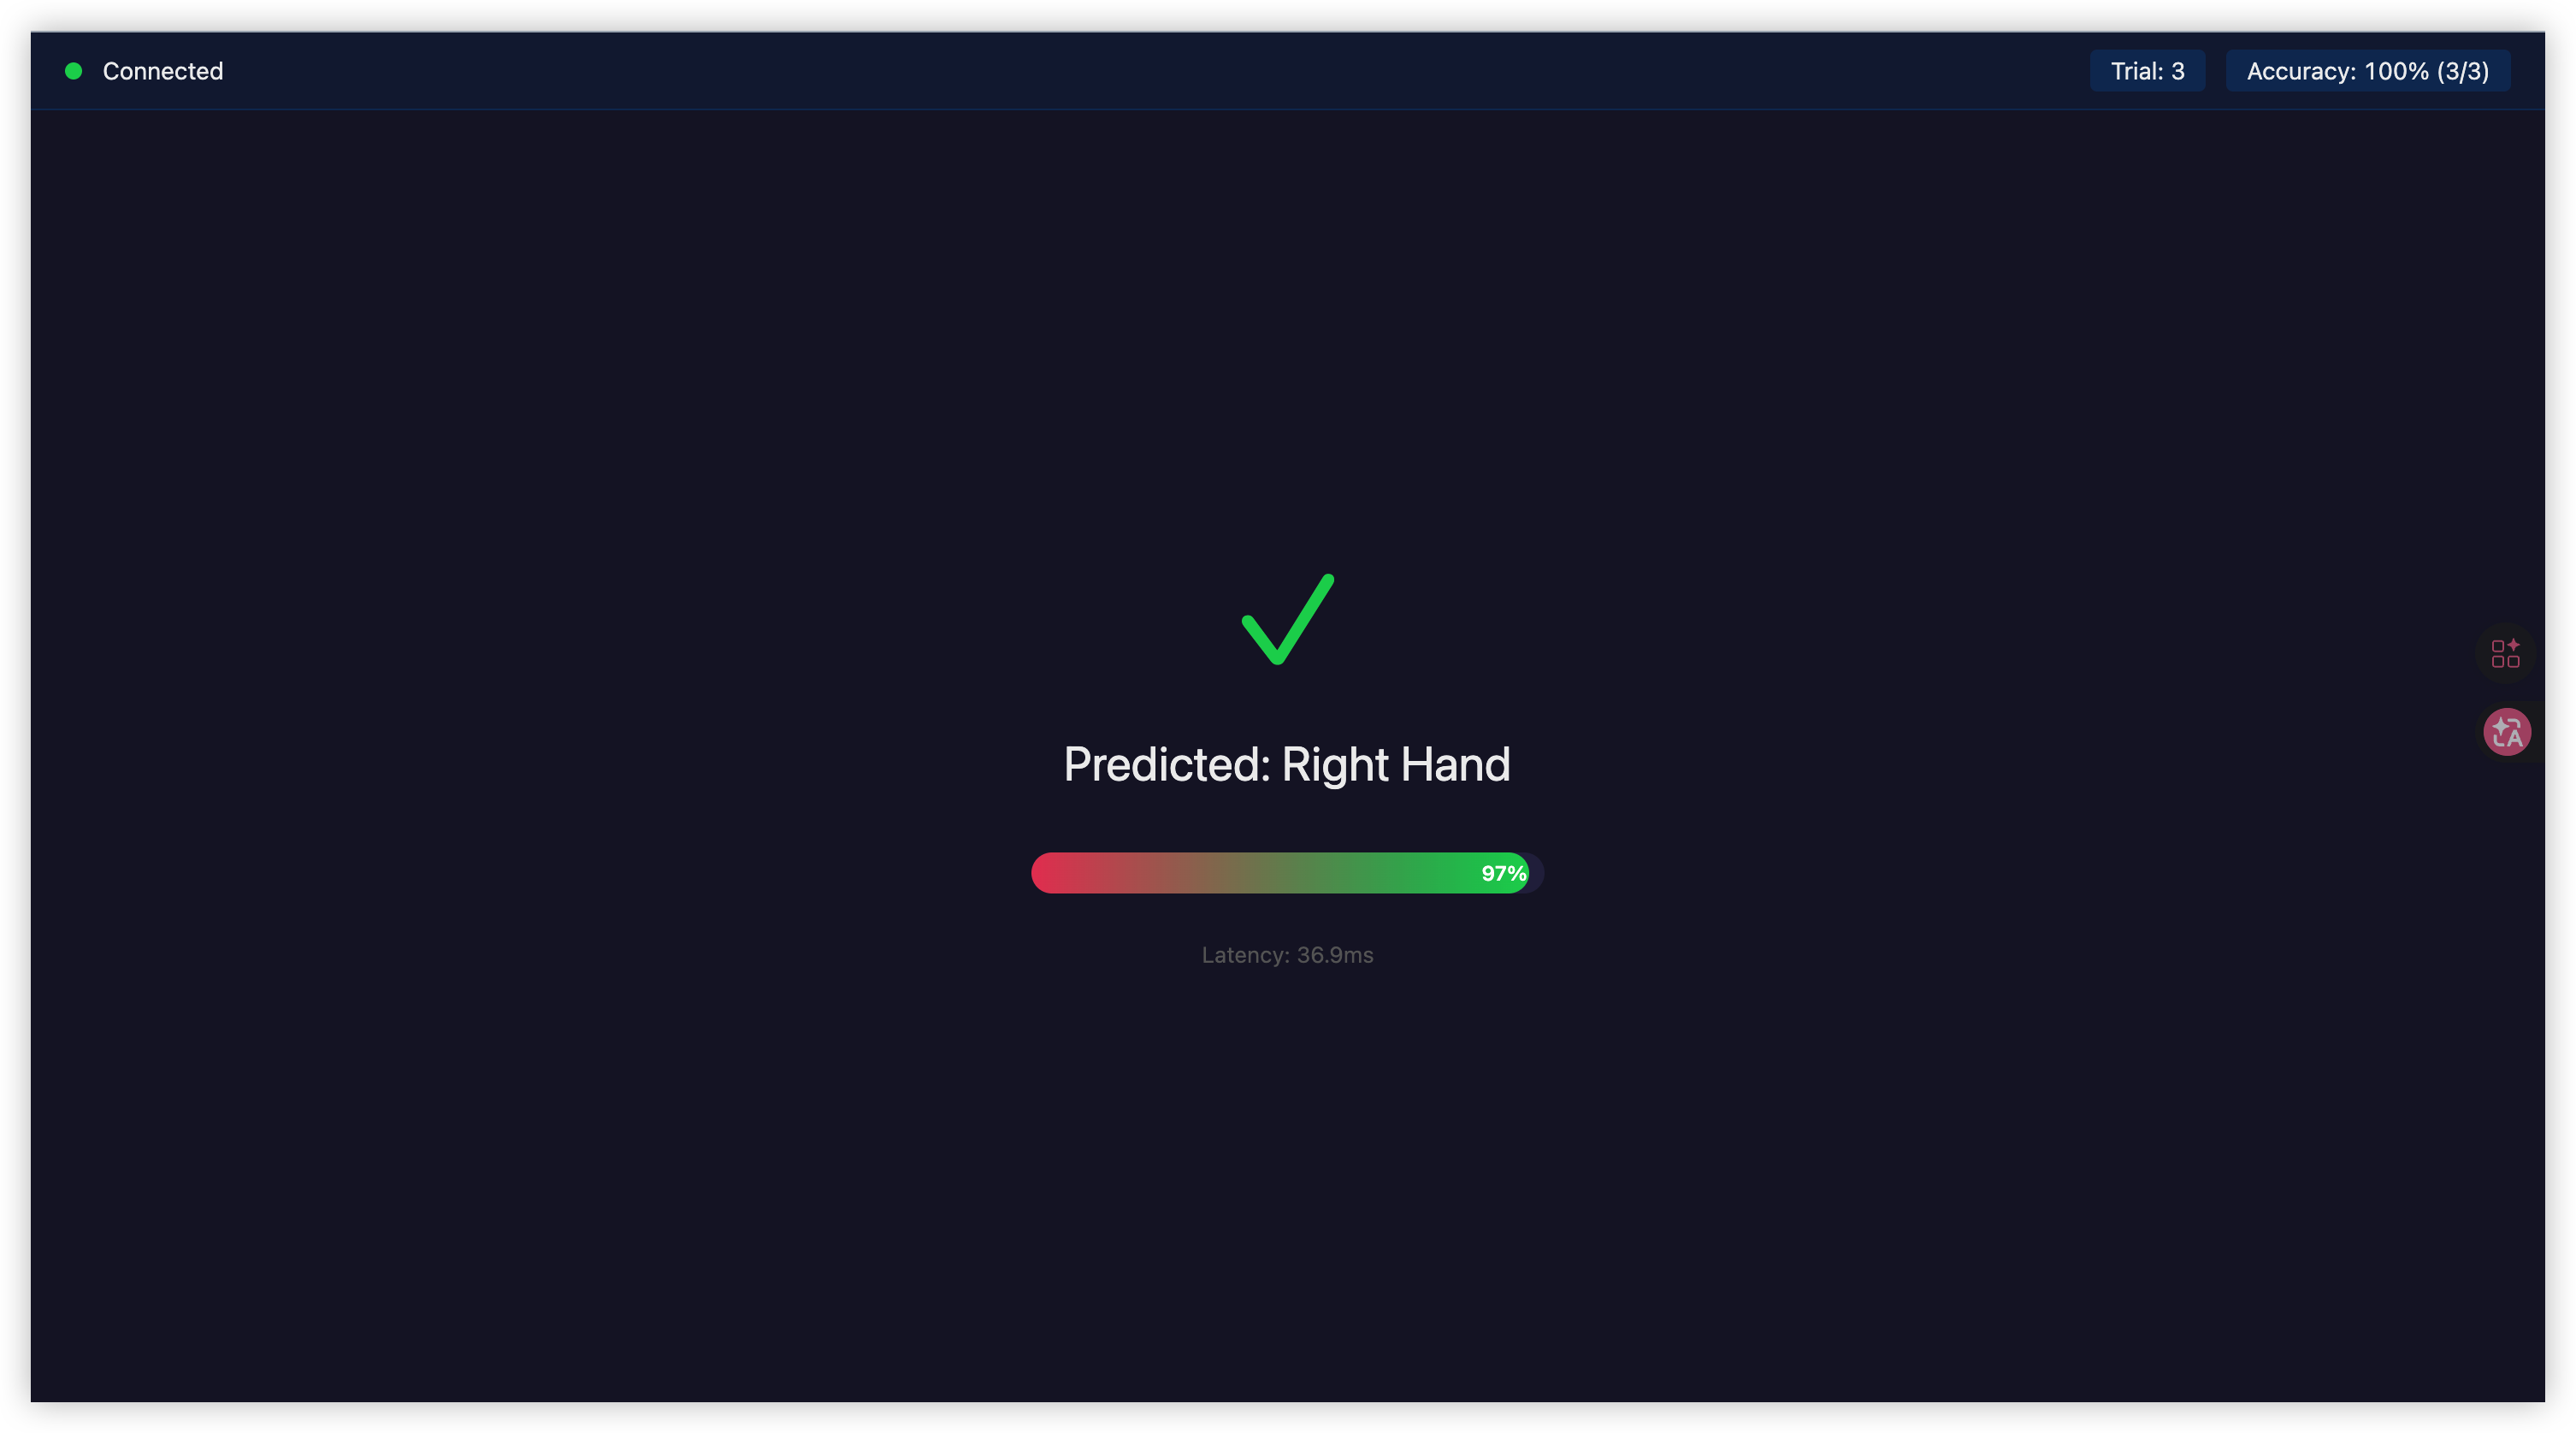
\includegraphics[width=0.85\textwidth]{online.png}
	\bicaption{在线仿真系统浏览器前端截图（feedback 状态）\label{fig:online-screenshot}}{Browser frontend screenshot of the online simulation system (feedback state)}
\end{figure}

% -------------------------------------------------------------------
\subsection{系统性能测试}
\label{sec:online-performance}
% -------------------------------------------------------------------

\subsubsection{分类延迟}

在线分类延迟是从接收 epoch 数据到输出预测结果的耗时，包含 FBCSP 特征提取和 SVM 预测两个步骤。表\ref{tab:online-latency}给出了在被试1数据上的延迟统计。

\begin{table}[htbp]
	\centering
	\bicaption{在线分类延迟统计（被试1，144 试次）\label{tab:online-latency}}{Online classification latency statistics (Subject 1, 144 trials)}
	\begin{tabular}{cccc}
		\toprule
		指标 & 均值 & 最小值 & 最大值 \\
		\midrule
		分类延迟 & 36\,ms & 24\,ms & 48\,ms \\
		\bottomrule
	\end{tabular}
\end{table}

平均 36\,ms 的分类延迟远低于 BCI 系统通常要求的 200\,ms 上限\upcite{wolpaw2002bci}，证明 FBCSP+SVM 方案完全满足实时性需求。相比之下，如果使用 EEGNet 进行在线推理，单试次 GPU 推理延迟约为 5--10\,ms（不含数据传输），但 CPU 推理可达 50--100\,ms，且需要额外的 PyTorch 运行时开销——这是第六章选型时排除 EEGNet 的又一工程理由。

\subsubsection{在线分类准确率}

在线仿真使用与离线评估相同的预处理后数据，因此在线准确率应与离线交叉验证结果一致。实测被试1的在线准确率为 92.4\%（133/144 试次正确），与离线 FBCSP+SVM 的 92.3\% 吻合（差异来源于在线模式使用全量训练数据而非交叉验证分折）。

\subsubsection{通信性能}

WebSocket 通信的单条 JSON 消息大小约 200--500 字节，在局域网环境下传输延迟 $<$ 1\,ms，对整体系统延迟的贡献可以忽略。HTTP 静态文件服务在首次加载后全部缓存于浏览器，不产生持续网络开销。

% -------------------------------------------------------------------
\subsection{本章小结}
% -------------------------------------------------------------------

本章基于第六章的 FBCSP+SVM 算法选型结论，实现了完整的在线 BCI 仿真系统。系统采用数据回放 + WebSocket + 浏览器的三层架构，通过试次状态机驱动"提示 → 想象 → 分类 → 反馈 → 休息"的闭环流程。后端平均分类延迟 36\,ms，远低于实时性要求（$<$ 200\,ms）；在线准确率与离线评估一致（被试1: 92.4\%），验证了从离线模型到在线部署的无损迁移。该系统为未来接入实时 EEG 采集设备提供了可直接复用的软件框架。


% ===================================================================
\section{总结与展望}
\label{sec:conclusion}
% ===================================================================

% -------------------------------------------------------------------
\subsection{本文工作总结}
% -------------------------------------------------------------------

本文围绕"基于脑电运动想象的脑机接口系统"展开研究，完成了以下主要工作：

\textbf{（1）构建了完整的 EEG 信号处理与分类系统。}从原始 EEG 数据出发，实现了包含共平均参考、带通滤波、ICA 伪迹去除、事件分段和坏段拒绝的标准化预处理流水线（第四章）。在此基础上，搭建了 CSP+LDA、FBCSP+SVM 和 EEGNet 三条分类流水线（第五章），通过 YAML 配置系统实现实验的可复现管理（第三章）。

\textbf{（2）系统验证了 FBCSP+SVM 的分类优势。}以 BCI Competition IV Dataset 2a 为主实验数据集，采用 10 折分层交叉验证进行评估（第六章）。结果表明：FBCSP+SVM 取得 82.2\% 的平均准确率（$\kappa = 0.645$），相比 CSP+LDA 基线（78.7\%）提升 3.5 个百分点，相比 EEGNet（72.6\%）提升 9.6 个百分点。跨数据集全局 Friedman 检验证实三种方法间存在高度显著差异（$p = 1.29 \times 10^{-4}$）；Wilcoxon 检验证实 EEGNet 在多通道数据集上显著弱于传统方法。在 Dataset 2b 和 PhysioNet EEGBCI 两个验证数据集上，FBCSP+SVM 同样表现出与 CSP+LDA 可比或更优的性能，进一步证实了频带自适应机制的泛化有效性。

\textbf{（3）FBCSP 特征选择结果揭示了个体差异的频带来源。}互信息特征选择的子频带分布热力图（图\ref{fig:fbcsp-heatmap}）直观展示了不同被试依赖不同频率成分的现象：部分被试的判别信息主要来自 Mu 频段（8--12\,Hz），另一些则更依赖 Beta 频段（16--24\,Hz）。这一发现从数据层面验证了 FBCSP 相比固定频带 CSP 的理论优势。

\textbf{（4）实现了完整的在线 BCI 仿真系统。}基于 FBCSP+SVM 的选型结论，搭建了"数据回放 + WebSocket + 浏览器"三层架构的在线仿真系统（第七章）。系统通过试次状态机驱动"提示 → 想象 → 分类 → 反馈 → 休息"的闭环流程，后端平均分类延迟 36\,ms，远低于 200\,ms 的实时性要求；在线准确率（被试1: 92.4\%）与离线评估结果（92.3\%）一致，验证了从离线模型到在线部署的无损迁移。

% -------------------------------------------------------------------
\subsection{不足与局限}
% -------------------------------------------------------------------

本文工作存在以下不足之处：

\textbf{（1）未使用实时 EEG 采集硬件。}本文的在线仿真系统基于离线数据的回放，尚未接入真实 EEG 放大器进行实时采集与处理。回放数据已经过离线预处理，因此无法反映实际在线场景中的信号质量波动、采集设备延迟和实时预处理的计算开销。

\textbf{（2）仅实现二分类任务。}本文聚焦于左手/右手两类运动想象的二分类问题，尚未扩展到 Dataset 2a 原始支持的四分类（左手、右手、双脚、舌头）。四分类场景下 CSP 需要采用 One-vs-Rest 或 One-vs-One 策略，FBCSP 的特征维度也将显著增加，算法性能和选型结论可能需要重新评估。

\textbf{（3）深度学习方法未充分发挥。}EEGNet 在本文的实验条件下（单被试、90--160 个试次）表现不佳，但这并不意味着深度学习在 MI-BCI 中没有潜力。本文未探索预训练-微调、数据增强、跨被试迁移学习等可能缓解小样本问题的深度学习策略。

\textbf{（4）缺乏跨被试和跨会话评估。}本文所有实验均为被试内交叉验证，未系统评估模型在不同被试之间或同一被试不同时间会话之间的泛化能力。跨被试/跨会话性能的下降是 MI-BCI 走向实际应用的关键瓶颈。

% -------------------------------------------------------------------
\subsection{未来展望}
% -------------------------------------------------------------------

基于本文的工作基础，未来可在以下方向继续深入研究：

\textbf{（1）接入实时 EEG 采集设备。}本文已预留了在线系统的软件框架（数据接口、状态机、WebSocket 通信），未来可替换数据回放模块为实时 EEG 采集接口（如 Lab Streaming Layer），实现从仿真到实际硬件的系统升级。

\textbf{（2）迁移学习提升跨被试泛化。}可采用域自适应方法（如对齐协方差矩阵或深度域自适应网络）利用已有被试数据辅助新被试的模型校准，减少新被试所需的训练数据量，缓解 BCI illiteracy 问题。

\textbf{（3）在线自适应更新。}在 BCI 使用过程中，使用者的脑电特征会随时间发生漂移。可在在线系统中引入增量学习机制，根据反馈信号实时更新分类模型的参数，以维持长时间使用中的分类性能。

\textbf{（4）多分类扩展与 3D 可视化前端。}将当前二分类系统扩展为四分类，同时开发基于 Unity 3D 的沉浸式前端，通过三维场景中的物体运动（如虚拟手臂、光标导航）提供更直观的运动想象反馈。


\label{article}  % 请勿删除此行
